\documentclass[]{dukedissertation}
%\documentclass[economy,twoside,bind]{dukedissertation}
% Use the second for a single-spaced copy suitable for duplex printing
% and binding.

% Other useful options (there are more options documented in Chapter 2):
%  * draft -- don't actually include images, print a black bar on overful
%             hboxes
%  * MS    -- Format for a Master's Thesis.  No UMI abstract page, some 
%             textual changes to title page.  


% Useful packages for dissertation writing:
\usepackage{amsmath, amssymb, amsfonts, amsthm}
\usepackage{graphicx}
\usepackage{natbib}
\usepackage{color}
\usepackage{bm}
\usepackage{subfigure}
\usepackage{graphicx}
\usepackage{mathabx}
\usepackage{multirow}
\usepackage{setspace}
% \usepackage{cite}  % If you include this, hyperlink cites will
                     % break.  It's nice to use this package if your bibstyle
							% sorts entries by order-of-use, rather than
							% alphabetically (as plain does).
							
%Theorem, Lemma, etc. environments
\newtheorem{theorem}{Theorem}%[section]
\newtheorem{lemma}[theorem]{Lemma}
\newtheorem{proposition}[theorem]{Proposition}
\newtheorem{corollary}[theorem]{Corollary}
\newtheorem{result}[theorem]{Result}

% Personal commands and abbreviations.
%Define and personal commands here

%Graphics Path to find your pictures
\graphicspath{{./Pictures/}}


%-----------------------------------------------------------------------------%
% PREAMBLE 
%-----------------------------------------------------------------------------%
\author{[Your Name Here]}
\title{[Your Title Here]}
\supervisor{[Your Supervisor Here]}
\department{[Your Department Here]} % Appears as Department of \department
% Declare dissertation subject used on UMI abstract page.  List of
% categories: http://dissertations.umi.com/duke/subject_categories.html
%\subject{[Your Subject Here]}

\date{2011} % Anything but the year is ignored.

% Copyright text.  If undefined, default is 'All rights reserved'
% (Example sets the text to a hyperlinked Creative Commons Licence)
\copyrighttext{ All rights reserved except the rights granted by the\\
   \href{http://creativecommons.org/licenses/by-nc/3.0/us/}
        {Creative Commons Attribution-Noncommercial Licence}
}

% Committee Members other than supervisor.  No more than five beyond the
% supervisor allowed.
\member{[Department Committee Member \#1]}
\member{[Department Committee Member \#2]}
\member{[External Committee Member]}
%-----------------------------------------------------------------------------%


%-----------------------------------------------------------------------------%
% HYPERREF: plain black hypertext references for ref's and cite's.
%-----------------------------------------------------------------------------%
\usepackage[pdftex, pdfusetitle, plainpages=false, 
				letterpaper, bookmarks, bookmarksnumbered,
				colorlinks, linkcolor=black, citecolor=black,
	         filecolor=black, urlcolor=black]
				{hyperref}

\begin{document}

%-----------------------------------------------------------------------------%
% TITLE PAGE -- provides UMI abstract title page & copyright if appropriate
%-----------------------------------------------------------------------------%
\maketitle

%-----------------------------------------------------------------------------%
% ABSTRACT -- included file should start with '\abstract'.
%-----------------------------------------------------------------------------%
\abstract

Write your abstract here.  You should not include references or mathematical notation.
}

%-----------------------------------------------------------------------------%
% DEDICATION -- OPTIONAL.  Put the text inside the braces.
%               (Long 'dedications' probably belong in the acknowledgements)
%-----------------------------------------------------------------------------%
\dedication{If you want to dedicate your thesis to anyone do so here}

%-----------------------------------------------------------------------------%
% FRONTMATTER -- ToC is required, LoT and LoF are required if you have any
% tables or figures, respectively. List of Abbreviations and Symbols is 
% optional.
%-----------------------------------------------------------------------------%
\tableofcontents % Automatically generated
\listoftables	% If you have any tables, automatically generated
\listoffigures	% If you have any figures, automatically generated
\abbreviations

% You can put here what you like, but here's an example
%Note the use of starred section commands here to produce proper division
%headers without bad '0.1' numbers or entries into the Table of Contents.
%Using the {\verb \begin{symbollist} } environment ensures that entries are
%properly spaced.

\section*{Symbols}

Put general notes about symbol usage in text here.  Notice this text is
double-spaced, as required.

\begin{symbollist}
	\item[$\mathbb{X}$] A blackboard bold $X$.  Neat.
	% Optional item argument makes the symbol/abbr
	\item[$\mathcal{X}$] A caligraphic $X$.  Neat.
	\item[$\mathfrak{X}$] A fraktur $X$.  Neat.
	\item[$\mathbf{X}$] A boldface $X$.
	\item[$\mathsf{X}$] A sans-serif $X$. Bad notation.
	\item[$\mathrm{X}$] A roman $X$.
\end{symbollist}

\section*{Abbreviations}

Long lines in the \texttt{symbollist} environment are single spaced, like in
the other front matter tables.

\begin{symbollist}
	\item[AR] Aqua Regia, also known as hydrocloric acid plus a splash of 
	nitric acid.
	\item[SHORT] Notice the change in alignment caused by the label width
	between this list and the one above.  Also notice that this multiline
	description is properly spaced. 
	\item[OMFGTXTMSG4ME] Abbreviations/Symbols in the item are limited to
	about a quarter of the textwidth, so don't pack too much in there.
	You'll bust the margins and it looks really bad.
\end{symbollist}
} % List of Abbreviations. Start file with '\abbreviations'

%-----------------------------------------------------------------------------%
% ACKNOWLEDGEMENTS -- included file should start with '\acknowledgements'
%-----------------------------------------------------------------------------%
\acknowledgements

Thank anyone you like here.  It's good practice to thank every granting agency that's given you money
since you've been ABD, any other school you visited during your research,
and any professional society that's funded your travel.
}

%==============================================================================
%-----------------------------------------------------------------------------%
%
% MAIN BODY OF PAPER
%
%
%-----------------------------------------------------------------------------%
\chapter{Motivations}

Cancer is considered to be the second biggest killer after cardiovascular diseases: there were an estimated 14.1 million cancer cases around the world in 2012, of these 7.4 million cases were in men and 6.7 million in women. This number is expected to increase to 24 million by 2035 \cite{Ferlay2012}.

Although surgery remains the most diffuse and successful treatment, radiotherapy is an important and effective option used for curative and palliative management of malignant tumors.
In approximately the $50\%$ of clinical cases, radiation therapy is a part of the initial treatment and it is usually conducted by means of high-energy X-rays \cite{Durante2010}.

Results of radiotherapy are improved when a high dose of radiation with high biological effectiveness is delivered to the tumour with the least possible dose to the surrounding tissues, especially in the case of critical organs \cite{Linz2011}.
In order to increase the conformity of the dose delivered to the tumour, diverse technologies have been considered and used.
Traditional forms of radiotherapy, X-ray tubes (energy $\sim$ 100 keV) or radioactive isotopes, have been replaced by linear accelerator delivering ($\sim$ 10 MeV) from different directions (e.g. Intensity Modulated Radio Therapy).
Although being widely used as a standard in radiation therapy, the effectiveness of conventional electromagnetic radiation is limited by the intrinsic characteristics of interaction with matter.
With respect to this, the scientific community is focusing its attention towards possible improvements of ion beam therapy \cite{Amaldi2011}.
In particular two aspects disfavours the usability of electromagnetic radiation with respect to ion for tumour targeting: the depth dose profile, which does not allow for an optimal dose deposition to the tumour sparing vital organs,
and the inferior biological effectiveness, which is the limiting factor in case of radio resistant tumours.
Heavier charged particles, like protons and ions (He-Ca) have the potentiality to overcome the limits of conventional therapy. 
As explained in the next section, ion beam therapy is more effective for targeting deep lying  or inoperable tumours.
The issues connected to range uncertainties require the development of an effective imaging technique for beam monitoring. 
Since this thesis is focused on the operational parameters of one of these techniques, Time-Of-Flight Positron Emission Tomography, a brief introduction of ion beam techniques and in-vivo monitoring is given in this chapter.

\begin{figure}
\centering
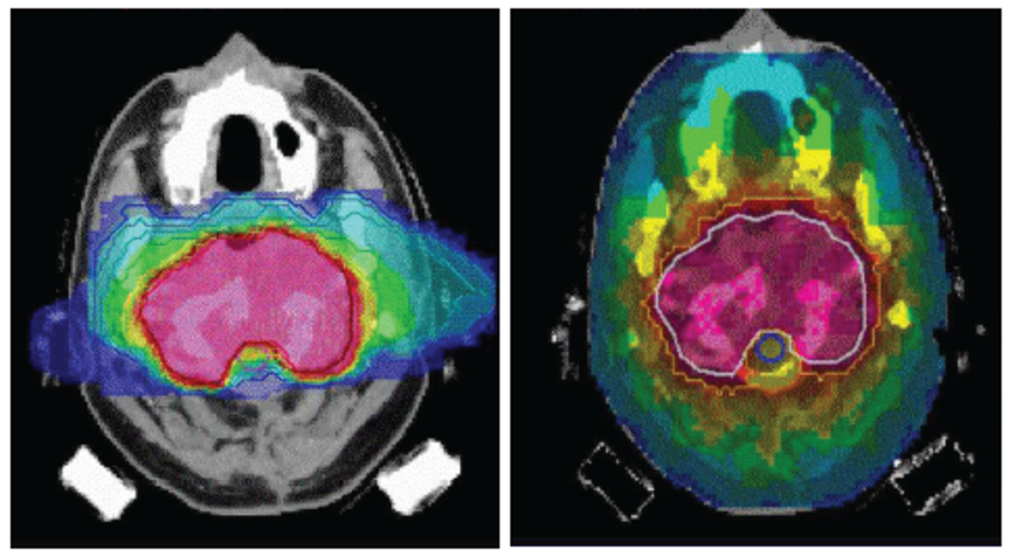
\includegraphics[width=12cm]{Pictures/Chapter_1/treat_conf2.pdf}
\caption[X-ray and proton irradiation]{Comparison of treatment plans for a large target volume in the base of the skull. Plan for carbon ions (left) and IMRT (right) \cite{Durante2010}.}
\label{fig:irradiation}
\end{figure}

\section{Particle therapy}
\subsection{Ion beam therapy}

The first proposition of ion beam therapy was presented in 1946 by R. Wilson \cite{Wilson1946}. The original idea was to exploit the physical properties of ion interaction in matter to improve the precision in radiotherapy treatments.  
Making use of the so called Bragg peak, that is using the fact that protons and ions in general deposit a maximum of energy at the end of their trajectory, the treatment could save the surrounding tissue from radiation overdose.

\begin{figure}
\centering
\begin{subfigure}
  {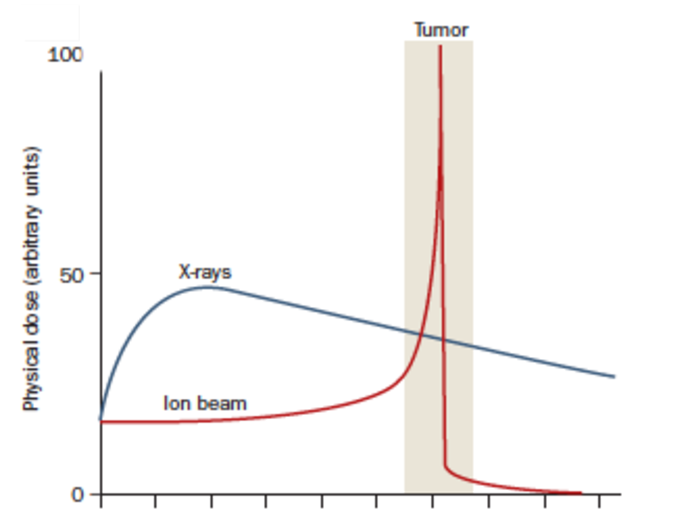
\includegraphics[width=6cm]{Pictures/Chapter_1/profile.pdf}}
\end{subfigure}
\begin{subfigure}
  {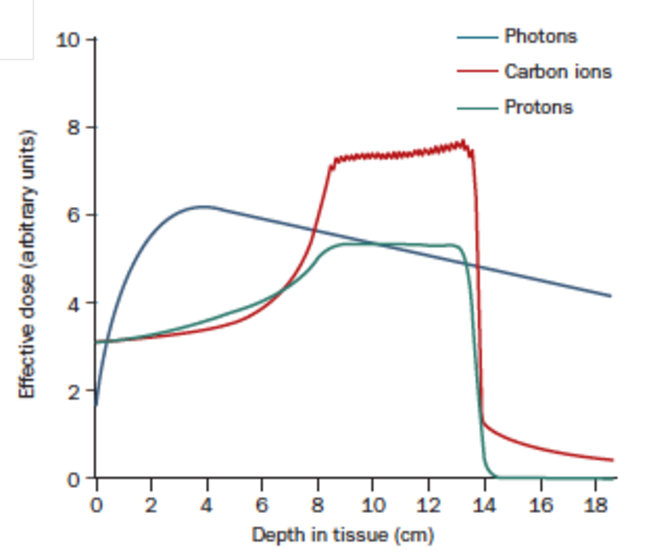
\includegraphics[width=6cm]{Pictures/Chapter_1/SOBP.pdf}}
\end{subfigure}
\caption[Depth dose comparison]{Comparison of the depth–dose relationships for X-rays and high-energy charged particles. In treatment of large tumors, the Bragg peak must be broadened by use of overlapping beams with different energies \cite{Durante2010}.}
\label{fig:test}
\end{figure}

The dose deposited by photons, considered as the gold standard for tumour treatment, is maximum close to the beginning of the trajectory in the body and is characterized by an exponential decrease. As a consequence, an undesired radiation dose is delivered to healthy tissues around the targeted tumour.

The recent therapeutic interest of ions in the field of radiotherapy relies mainly on their high relative biological effectiveness.
LET (linear energy transfer) has long been viewed as the main parameter to discern the biological effect of different kinds of radiation. It is a measure for the energy deposited by a charged particle traveling through matter. LET is closely related to stopping power and is not a constant value, since it changes along the particle's path (es 10 KeV/$\mu$m for photons, 100 KeV/$\mu$m for protons, 1000 KeV/$\mu$m for ions).
When considering ions of different atomic number LET becomes a limited parameter to evaluate the biological effect. 

In this sense the relative biological effectiveness (RBE) is considered the most accurate quantity, since it is defined as the biological effect of one type of ionizing radiation relative to another, given the same amount of absorbed energy. As the charge of the incident ions increases, so does the probability of severe DNA damage. An elevate RBE in the Bragg peak region has clearly been demonstrated for ions heavier than Helium  \cite{Linz2011}.
As a consequence they prove to be more effective for targeting radio resistant or inoperable tumours.

%rbe
\begin{figure}  
\centering
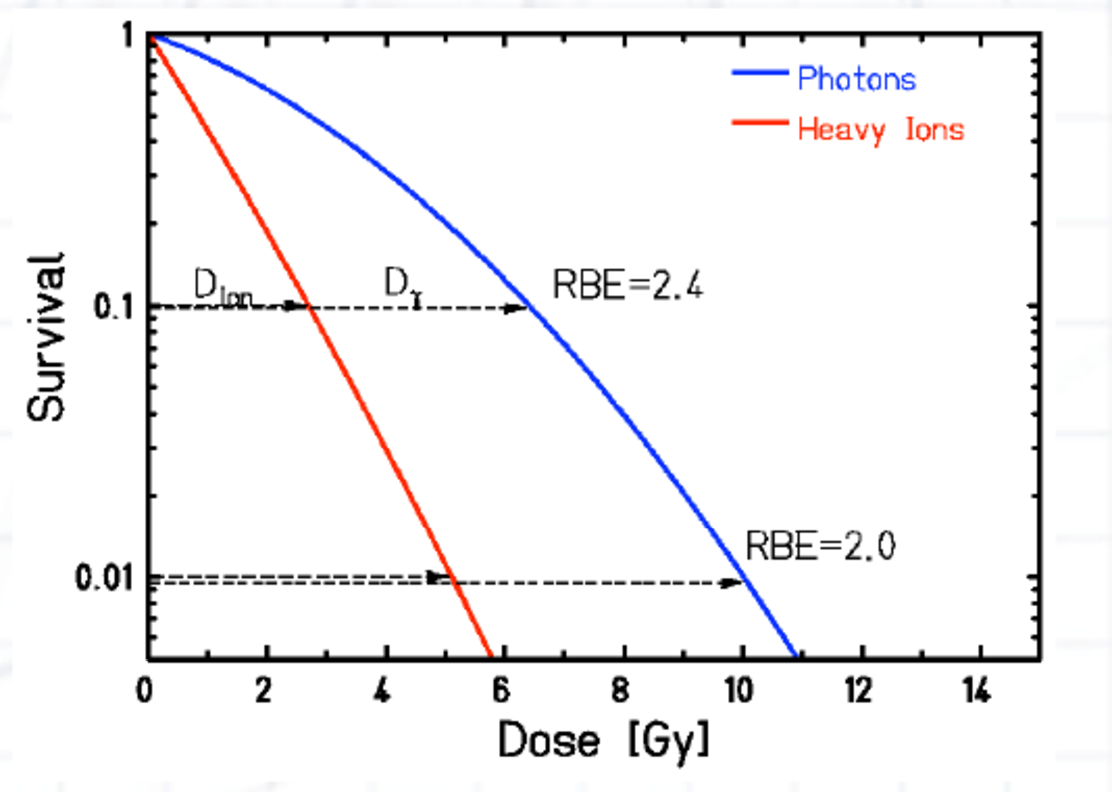
\includegraphics[width=8cm]{Pictures/Chapter_1/rbe.pdf}
\caption[RBE comparison]{Comparative plot of RBE for photons and heavy ions.}
\label{fig:rbe}
\end{figure}

\subsection{Beam delivery}

Ion beams are delivered by either cyclotrons or synchrotrons. In the first case the beam has a fixed energy which is tuned by means of degraders in order to deliver the correct dose profile. In the case of synchrotron the beam is delivered in spills and the energy is varied between spills. In the case of Carbon only synchrotrons can be used.
To deliver the dose to the planned target volume (PTV) different energies are superimposed in order to obtain the so-called spread-out Bragg peak (SOBP). The beam is usually delivered in a passive beam shaping setup or a scanning system. 

Different sources of error can worsen the dose delivery profile, such as patient mis positioning and evolution of the tumour/morphology of the patient. In addition the complex physics of ion interaction leads to  imprecisions in the treatment plannings, due to fragmentation of the incident beam and range uncertainties.

Usually treatment planning systems cope with these problems by irradiating a volume larger than the tumour itself, called planning target volume (PTV) which contains the clinical target volume (CTV). Complex compensating systems, including x-ray imaging techniques and patient positioning systems, allow to reduce errors in the dose profiles delivered. 
Treatment plannings of ion therapy rely for example on accurate values of particle range in tissue obtained from Hounsfield unit of computed tomograms, leading to uncertainties of $1-3\%$ in range calculations \cite{Enghardt2004}.

The dose delivered by a ion beam system is much more sensitive to these deviations than the one delivered by a photon beam. Due to the high biological effectiveness of ion beams, wrong ranges could lead to dramatic under dosage to the tumour or over dosage to organ at risk surrounding.
As a consequence a three-dimensional non invasive imaging technique for ion beam therapy monitoring is required. Since ions, unlike photons, are stopped completely in the patient volume, technology like portal imaging are not suitable. The attention of the community is thus focused on positron emission tomography (PET), which relies on the peculiar characteristics of $\beta ^{+}$ decay.

%prblemi di deliver
\begin{figure} 
\centering 
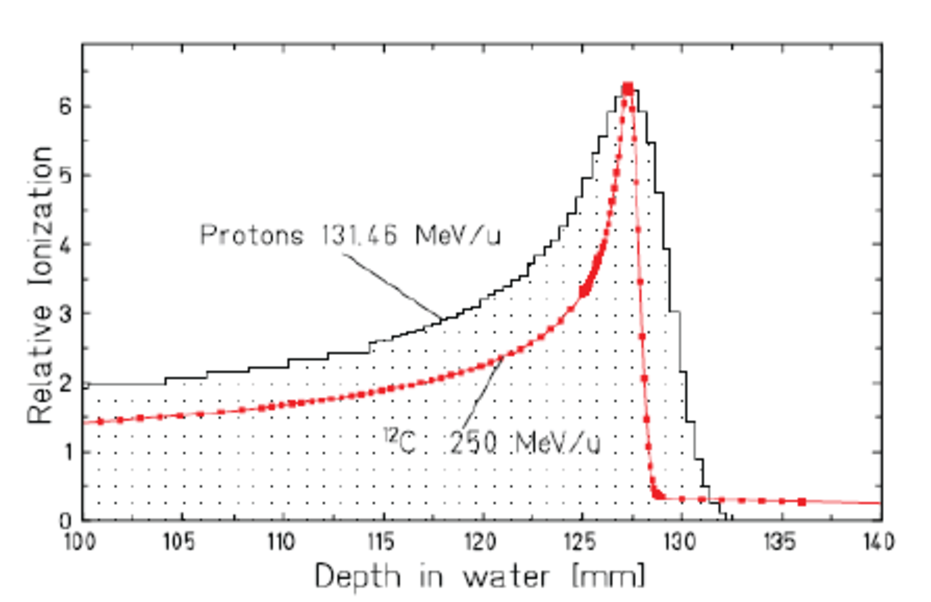
\includegraphics[width=8cm]{Pictures/Chapter_1/range_scatter.pdf}
\caption[Peak spread for Carbon]{Bragg curves of proton and C-ions having the same mean range (water phantom and ionization chamber) \cite{Schardt2007}.}
\label{fig:spread}
\end{figure}

\subsection{Monitoring of the beam}

Several attempts have already been undertaken to systematically assess the benefit of the PET method for beam monitoring, the principal one being the set up installed at the experimental carbon ion therapy unit at the Gesellschaft fur Schwerionenfroschung Darmstadt (GSI) \cite{Parodi2004}.
Two alternatives can be considered: the use of positron radioactive ions as projectiles for dose delivery or the detection of $\beta ^{+}$ activity given by nuclei fragmentation.
As an example of the first approach it is interesting to consider the effort made at the Heavy Ion Accelerator in Chiba (Japan), where radioactive beams of $^{11}C - ^{10}C$ ions deliver an activity of $10^{3} - 10^{5}$ $Bq$ $Gy^{-1}$ cm$^{-3}$ within the irradiated volume.
Due to the low production rate of secondary radioactive ions, this approach has been only partially successful.

Another possibility is to make use of the $\beta ^{+}$ activation given by the fragmentation of stable ions interacting with the tissue.
The radioactivity is a direct product of the irradiation and, although the activity density is rather low (around 600 $Bq$ $Gy^{-1}$ cm$^{-3}$ for protons), this method provides a rather cheaper and feasible solution \cite{Enghardt2004}.
The activity slides very fast under a reasonable threshold for detectability and the most effective solution is an in-beam scanner.
In-beam PET is currently the main method implemented clinically for in situ monitoring of charged hadron radiotherapy \cite{Crespo2007}.

% attivita irraggiamento!!!!!

%\begin{figure}  
%\includegraphics[width=\textwidth]{Pictures/Chapter_1/conformal_x_rays}
%\caption[Short figure name.]{Schematic view of depth-dose distributions of photons and ions. (a) photon
%field, (b) spread-out ion beam, (c) depth–dose profiles along the central beam axis \cite{Linz2011}.}
%\label{fig:myInlineFigure}}
%\end{figure}

\section{Positron Emission Tomography}
\subsection{Principles}
Positron Emission Tomography (PET) has been introduced as a nuclear medicine imaging technique which measures the distribution of a positron-emitting radionuclide (tracer), which is injected into the body on a biologically active molecule. In the case of in-beam PET the activity is present in the body of the patient due to the activation induced by proton interaction.

After the injection, or during the dose delivery, the subject of a PET study is placed within the field of view (FOV) of a number of detectors capable of registering incident $\gamma$ rays. The radionuclide in the radio tracer decays and the resulting positrons subsequently annihilate with electrons after travelling a short distance ($\sim$ 1 mm) within the body.

Each annihilation produces two $511$ keV photons travelling in opposite directions and these photons may be interact with detectors surrounding the subject. The detector electronics are linked so that two detection events unambiguously occurring within a certain time window may be called coincident and thus be determined to have come from the same annihilation. These events can be stored in arrays corresponding to projections through the patient and reconstructed using standard tomographic techniques. The resulting images show the tracer distribution throughout the body of the subject. The scheme of a PET scanner is shown in figure  \ref{fig:PET}.

As already mentioned, positron emission tomography relies on the $\beta ^{+}$ decay of a radionuclide.
% pet schema
\begin{figure}
\centering  
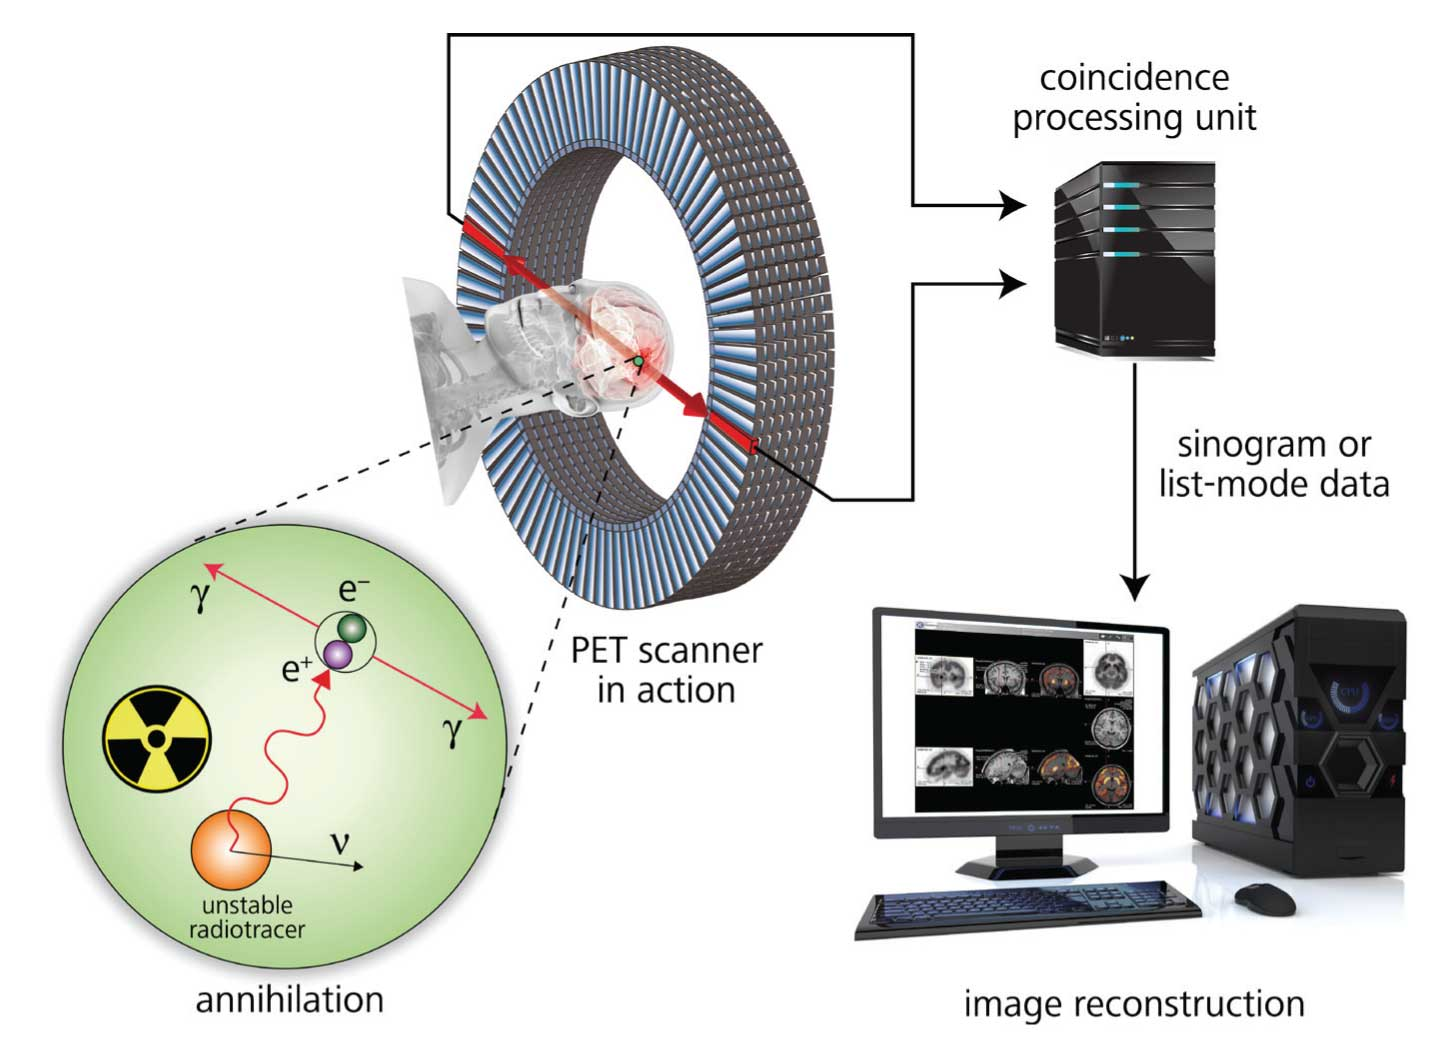
\includegraphics[width=8cm]{Pictures/Chapter_1/PET_scheme}
\caption[PET scanner]{Schematic view of PET scanner.}
\label{fig:PET}
\end{figure}
The nucleus of the radionuclide can convert a proton into a neutron 
\begin{displaymath}
p\rightarrow n + e^{+} + \nu _{e}
\end{displaymath}
As positrons travel through human tissue, they give up their kinetic energy principally by Coulomb interactions with electrons. As the rest mass of the positron is the same as that of the electron, the positrons may undergo large deviations in direction with each Coulomb interaction, and they follow a tortuous path through the tissue as they give up their kinetic energy.

When the positrons reach thermal energies, they start to interact with electrons either by annihilation, which produces two $511$ keV anti-parallel photons, or by the formation of a hydrogen-like orbiting couple called positronium. In its ground-state, positronium has two forms: ortho-positronium, where the spins of the electron and positron are parallel, and para-positronium, where the spins are anti-parallel. Para-positronium again decays by self-annihilation, generating two anti-parallel $511$ keV photons. Ortho-positronium self-annihilates by the emission of three photons. Both forms are susceptible to the pick-off process, where the positron annihilates with another electron. Free annihilation and the pick-off process are responsible for over $80\%$ of the decay events.

\subsection{Image reconstruction}

After all corrections have been applied to the data acquired, the number of counts assigned to a LOR joining a pair of crystals is proportional to a line integral of the activity along that LOR. Parallel sets of such line integrals are known as projections.
These projections are usually graphically represented as a sinogram, which collects the intensity valuesof the voxels in the coordinate system of variables $\phi$ and s, as shown in figure \ref{fig:reco}.

For image reconstruction, the most commonly used algorithms are the analytical method called filtered back projection and iterative reconstruction schemes.
% sinogram reco
\begin{figure} 
\centering 
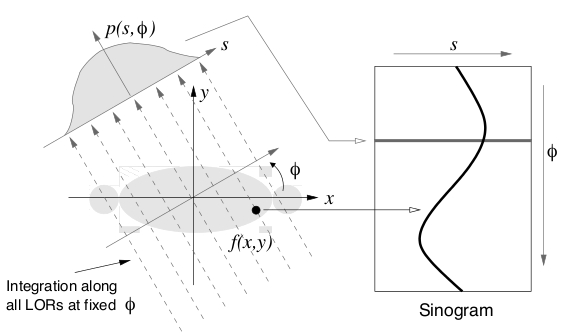
\includegraphics[width=8cm]{Pictures/Chapter_1/proj_sin.jpg}
\caption[Image reconstruction in PET]{Extraction of a sinogram from a 2D acquisition.}
\label{fig:reco}
\end{figure}
In particular iterative methods are often preferred over analytical approaches because they can account more effectively for the noise structure and can use a more realistic model of the system. Moreover advances in computation speed and faster algorithms allowed iterative methods to receive growing clinical acceptance.
An iterative method has five basic components.
\begin{itemize}
\item A model for the image, that is a discretization of the image domain into pixels (2-D) or voxels (3-D) or other exotic models.
\item A system model that relates the image to the data. A system model M is characterized by elements $M_{ij}$ related to the image system that represent the probability that an emission from voxel j is detected in projection i
\item A model for the data which describes the statistical relation between the value obtained and the value expected
\item A governing principle that defines the parameters of a "best" image, often expressed as a cost function (e.g. Maximum likelihood)
\item An algorithm that optimizes the cost function.
\end{itemize}

This last issue has been implemented in several ways, ranging from gradient-based algorithms to the commonly used Expectation Maximization (EM) algorithm and its variations (OSEM).

\subsection{Sources of noise and sensitivity}
In a PET scanner, each detector generates a timed pulse when it registers an incident photon. These pulses are then combined in coincidence circuitry, and if the pulses fall within a short time-window, they are deemed to be coincident.
A coincidence event is assigned to a line of response (LOR) joining the two relevant detectors. In this way, positional information is gained from the detected radiation without the need of a physical collimator. This is known as electronic collimation.
When a physical collimator is used, directional information is gained by preventing photons which are not normal or nearly normal to the collimator face from falling on the detector. In electronic collimation, these photons may be detected and used as signal.
Coincidence events in PET fall into four categories: true, scattered, random and multiple, as shown in figure \ref{fig:coinc}. 

True coincidences occur when both photons from an annihilation event are detected by detectors in coincidence, neither photon undergoes any form of interaction prior to detection, and no other event is detected within the coincidence time-window.

% coincidenze
\begin{figure}  
\centering
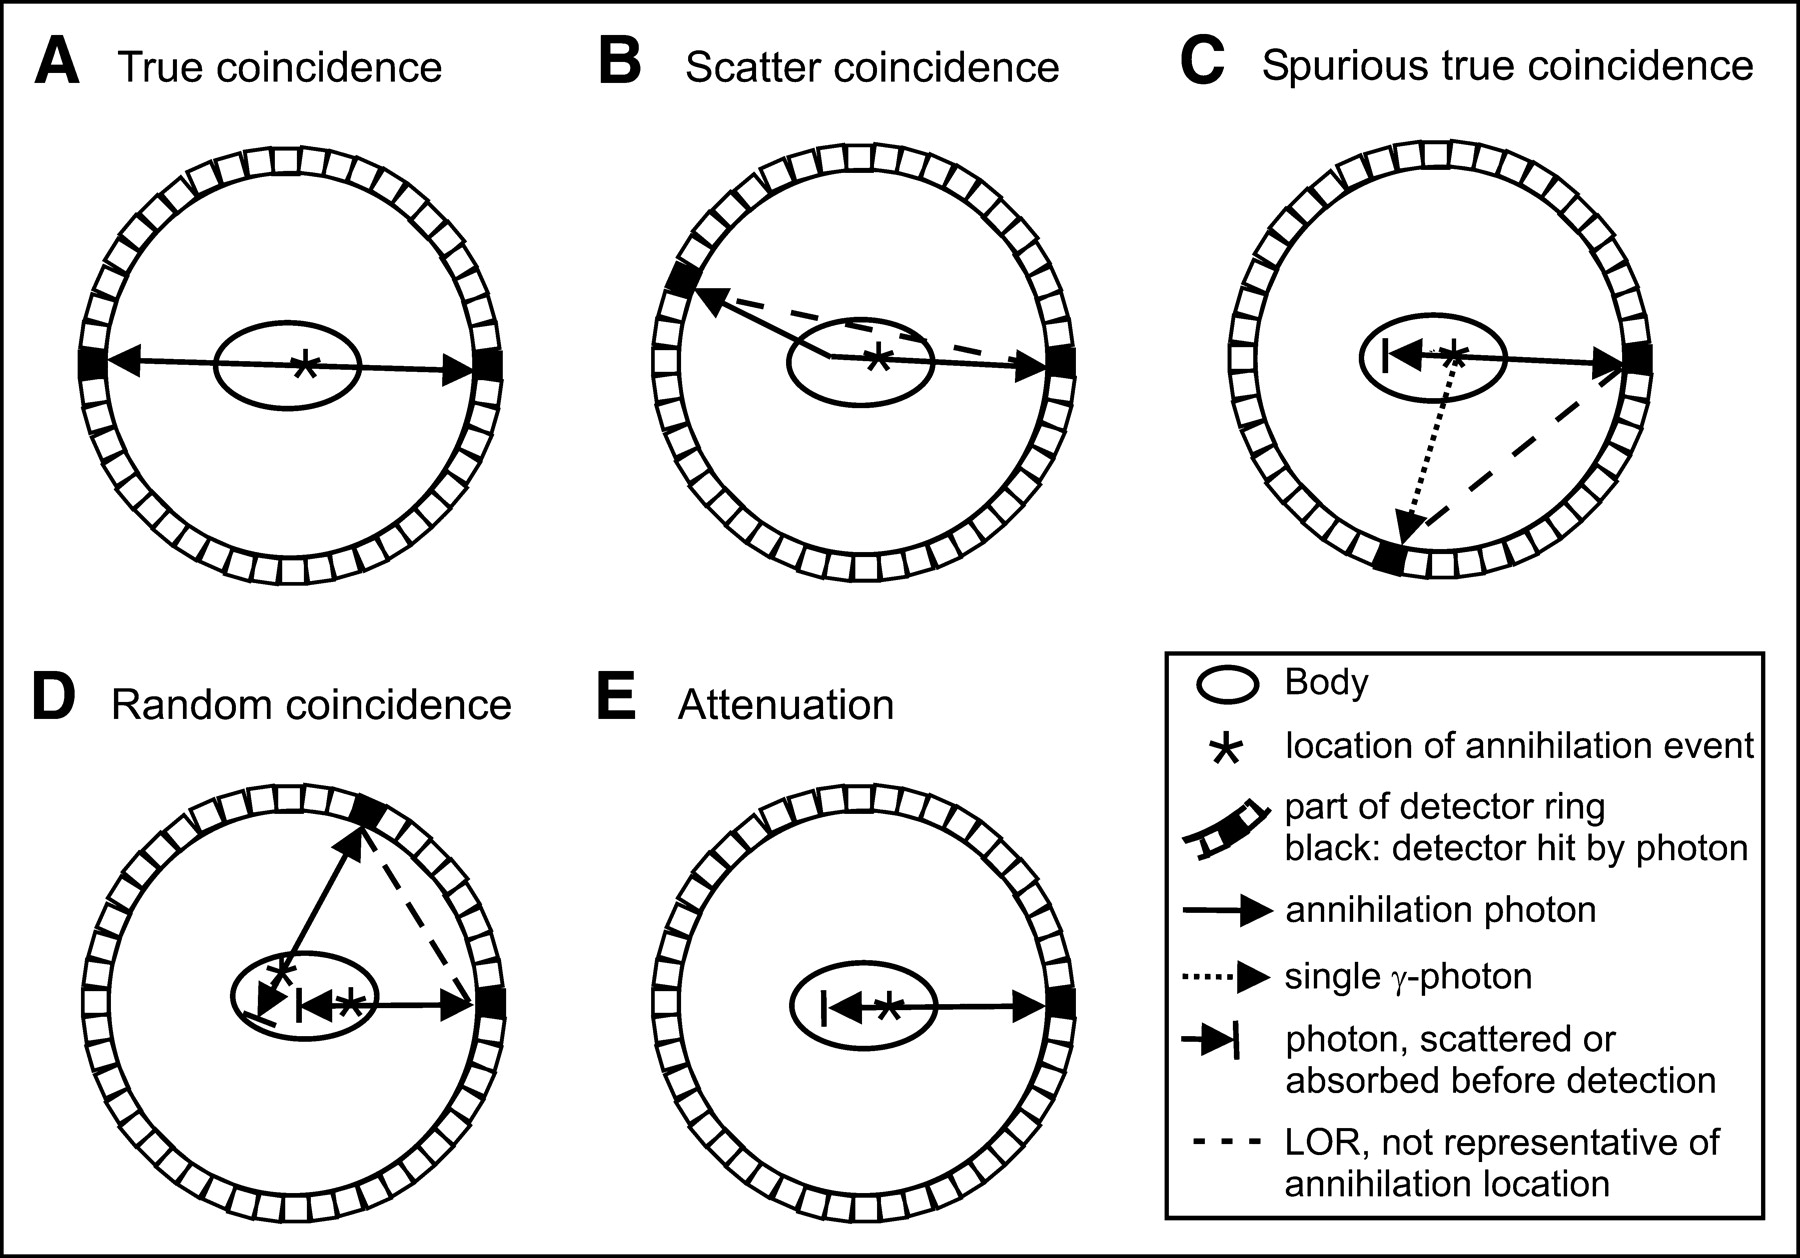
\includegraphics[width=8cm]{Pictures/Chapter_1/coinci_PET}
\caption[Coincidencies in PET exam]{Phenomelogy of PET examination. The cases b, c, d lead to loss of resolution.}
\label{fig:coinc}
\end{figure}

A scattered coincidence is one in which at least one of the detected photons has undergone at least one Compton scattering event prior to detection. Since the direction of the photon is changed during the Compton scattering process, it is highly likely that the resulting coincidence event will be assigned to a wrong LOR. Scattered coincidences add background to the true coincidence distribution which changes slowly with position, decreasing contrast and causing the isotope concentrations to be overestimated. They also add statistical noise to the signal. The number of scattered events detected depends on the volume and attenuation characteristics of the object being imaged, and on the geometry of the PET scanner.

Random coincidences occur when two photons not arising from the same annihilation event are incident on the detectors within the coincidence time window of the system. The number of random coincidences in a given LOR is closely linked to the rate of single events measured by the detectors joined by that LOR and the rate of random coincidences increase roughly with the square of the activity in the FOV. As with scattered events, the number of random coincidences detected also depends on the volume and attenuation characteristics of the object being imaged, and on the geometry of the scanner. The distribution of random coincidences is fairly uniform across the FOV, and will cause isotope concentrations to be overestimated if not corrected for. Random coincidences also add statistical noise to the data.
\newpage
\subsection{Time-Of-Flight PET}

It has been shown that in-beam PET could not provide definitive information to the oncologist when medium to large tumors are involved \cite{Fiedler2006}. This is due to the operative parameters of scanners available on the market, with relatively slow scintillators and tomographs covering small solid angles. A decisive improvement could be given by time-of-flight PET (TOF-PET).

Recent developments in scintillator technology and read out electronics allow to build detectors able to detect the time difference between the moment of detection of the opposed $\gamma$ rays in coincidence. 
%tof pet
\begin{figure}
\centering  
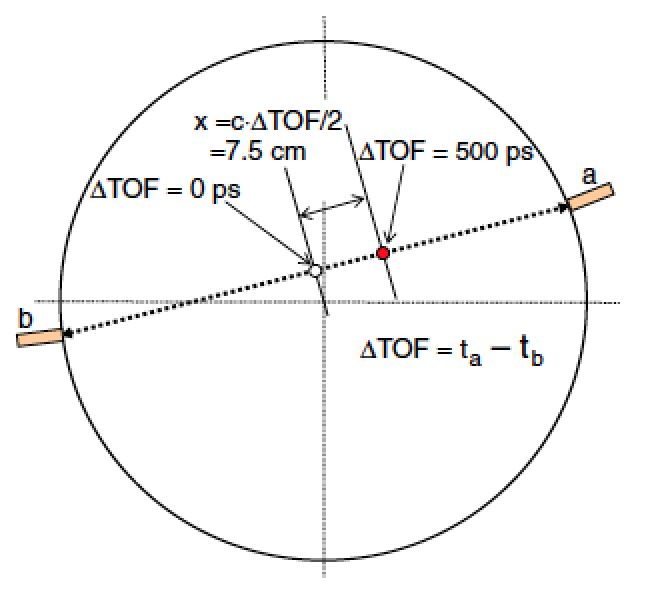
\includegraphics[width=6cm]{Pictures/Chapter_1/TOF}
\caption[TOF-PET schematics]{Example of time of flight information usage in PET examination.}
\label{fig:TOF}
\end{figure}
If we define a LOR between two detectors A and B, the distance between the center of the LOR and the annihilation point is given by
\begin{equation}
x = (t_{b}-t_{a} ) \cdot c/2
\end{equation}
where c is the speed of light. This situation is depicted in figure \ref{fig:TOF}.
Thus the spatial resolution is proportional to the coincidence time resolution (CTR) of the system.
Scanners available on the market today could deliver a 600 pico seconds time resolution, that translates to a positional uncertainty of 9 cm (FWHM) on the LOR.
The quality of the tomographic image largely benefits from the timing information of a TOF-PET scanner, since it reduces considerably  the contribution of Compton scattered photons and from photons from outside the field-of-view (FOV).
As a consequence the background from scattered and random coincidence is largely suppressed. 
The signal to noise ration (SNR) is thus dramatically improved, as we can write \cite{Karp2008}:
\begin{equation}
SNR \propto \frac{1}{\sqrt{n}}\left[ \frac{T^{2}}{T^{2} + S + R} \right]^{1/2}
\end{equation}
where where T representes the total trues, R thee random coincidences, S the scattered coincidence and n is the number of image elements contributing to a projection of the sinogram.
In the case of in-beam PET this is relevant, since it has been shown \cite{Fiedler2006} that during particle irradiation a considerable amount of activity is transported outside the FOV by metabolic processes. Moreover a high backround signal is typical of carbon ion beams \cite{Enghardt2004}. 
A useful and pratical estimation of the gain in signal to noise can be formalized as follows
\begin{displaymath}
G = \frac{SNR_{TOF}}{SNR_{non_{TOF}}} = \sqrt{\frac{2\cdot D}{c \cdot CTR}}
\end{displaymath}
where D is the diameter of the volume under examination, c is the speed of light and CTR is the coincidence time resolution. Thus a CTR of 100 ps FWHM translates into a 1.5 cm resolution on the position and a SNR gain of 5 (corresponing to a sensitivity gain of about a factor 25) compared to non TOF systems.

% quanto guadagni con tofpet
\begin{figure}  
\centering
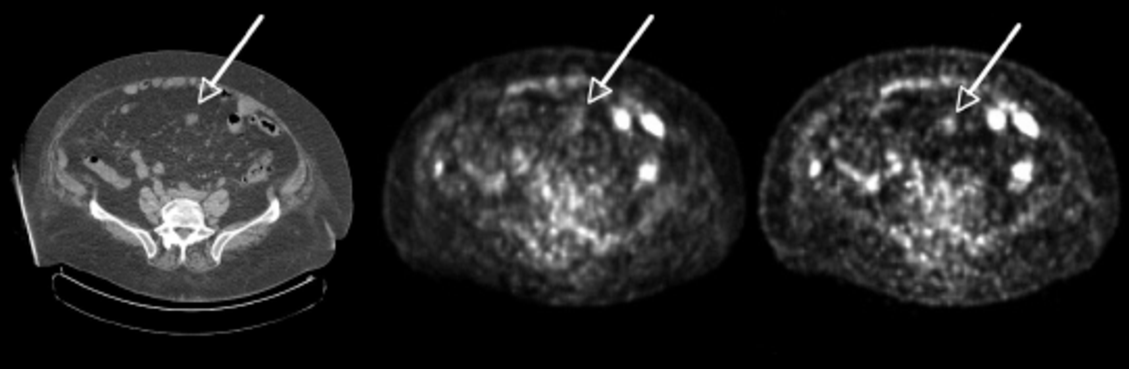
\includegraphics[width=14cm]{Pictures/Chapter_1/tof_gain.pdf}
\caption[Improvement of TOF-PET]{Representative transverse sections: low dose CT (left), non-TOF ML-EM (middle), and TOF ML-EM (right). The patient with colon cancer (119 kg, BMI = 46.5) shows a lesion in the abdomen seen in CT much more clearly in the TOF image than in the non-TOF image \cite{Karp2008}.}
\label{fig:tofgain}
\end{figure}

\section{Outline of the thesis}

\subsection{From high energy physics to medical applications}
The work outlined in these pages have been sponsored by \textit{The European training network in digital medical imaging for radiotherapy} (ENTERVISION) at the \textit{European Center of Nuclear Research} (CERN). ENTERVISION was established in February 2011 in response to the critical need for reinforcing research in online 3D digital imaging in order to deliver some of the key elements and building blocks for realizing the vision for early detection and more precise treatment of tumours.
The present work was hosted by CERN, the European Organisation of Nuclear Research, based in Geneva, Switzerland. 
CERN was established by a formal act in Paris, on 1st of July 1954, as an organisation that \textit{shall provide for collaboration among European States in nuclear research of a pure scientific and fundamental character, and in research essentially related thereto}.
Thourought its history, CERN provided experimental and theoretical tools to study and understand the fundamental forces governing our universe, in a continous effort to improve our understanding of elementary  physics. 

The ECAL detector at the CMS exeriment at the LHC was build with the fundamental contribution of the collaboration hosting this thesis: the Crystal Clear Collaboration. It was founded in 1990 as an international academic network of laboratories and industrial partners for the development of scintillating crystal detectors as well as their applications. It comprises experts in crystallography and solid state physics as well as in radiation detection and instrumentation. 
Its first goal was the development of a radiation-hard crystal for the ECAL detector, leading to the development of PbWO4 (PWO) as the material selected for CMS calorimeter. More recently the group has been focusing on the study of new materials for hadronic and electromagnetic calorimeters for future particle accelerators.
In parallel, the collaboration engaged in a effort of technology transfer to other domains exploiting the expertise developed in scintillating detectors. It is quite natural to focus the attention to medical physics, with particular respect to nuclear medicine since the requirements for detectors used in medical physics and detectors for high energy experiments are similar.

% high energy requirements
%\begin{figure}  
%\includegraphics[width=\textwidth]{Pictures/Chapter_1/conformal_x_rays}
%\caption[Short figure name.]{Schematic view of depth-dose %distributions of photons and ions. (a) photon
%field, (b) spread-out ion beam, (c) depth–dose profiles along the %central beam axis \cite{Linz2011}.}
%\label{fig:myInlineFigure}}
%\end{figure}

\subsection{Study of time profiles}

This thesis is devoted to the full characterization of the parameters that influence time resolution in a scintillator/photodetector setup, with particular attention focused on the impact of time profiles of heavy scintillators on the performance.

The first part of the presented work has the objective of describing the fundamental model that governs light production and collection in a PET-like setup.
In chapter 2 and 3 a brief introduction regarding heavy scntillator crystals and photodetectors is given.

With the objective of defining the operational parameters of our equipment, in chapter 3 a model based on multi-exponential time profiles has been implemented on an existing framework, widening the scope of usage by evaluating the role of Cerenkov photons produced by low energy radiation.

Moreover in order to properly characterized the operational parameters of a scintillator setup, a comparative analysis of ray tracing softwares has been conducted in chapter 5, namely the two packages SLitrani and Geant4. The latter has been chosen to build the simulation framework that allowed to disentangle the various source of resolution degradation.

Finally the work focused on the measurements and evaluation of rise time. Non zero rise time in scintillating systems is given by the different processes characterizing energy deposition inside a crystalline lattice, with utmost relevance of the latest stage of electron hole thermalization. The time scale of this phenomenon is $\sim$ 100 ps and until now has proven to be difficult to estimate due to the intrinsic limitations of detection setups.
Thus a time resolved study of different species of crystals is proposed in the final part of this work.
In chapter 6 the methodology followed is presented, from an experimental point of view and defining the main challenges of data analysis.
Finally the last two chapters present the time resolved study, with excitation energy varied from the 36 eV of a VUV femto second source to the 511 KeV of a $\gamma$ source. 


%\afterpage{\clearpage}


}

% cristalli in PET, Quenching, optical ( Rayleigh)

\chapter{Scintillating detectors}

In the field of medical applications, the energies of the $\gamma$ photons to be detected are usually of the order of hundreds of keV. In the case of PET scanners the energy of the two back to back photons is 511 KeV.
A simple approach to estimate the parameters of the incoming radiation is to make use of a fluorescent sample coupled to a photo detector. A standard setup would include a heavy scintillator crystal which converts the incoming radiation into visible photons. The following steps of the detection process involve transportation to the entrance window of the photodetector, conversion of the photons into an electric signal and subsequent manipulation of the signal by readout electronics.  

% schema rivelatore anzi no

\section{Interaction of radiation with matter}
In this work we are mainly concerned with the interaction of $\gamma$ radiation with matter, thus focusing our attention on the three existing mechanisms: photo electric interaction, Compton interaction and pair production.
Moreover electrons produced by ionizing interactions can polarize the medium, giving origin to the Cerenkov effect and producing visible photons, which can be of foremost importance in the case of timing application.

\subsection{Photoelectric effect}

In the case of the photoelectric effect an electron from an atom is freed upon absorption of the incoming photon:
\begin{equation}
\gamma + atom \rightarrow e^{-} + atom
\end{equation}
Due to conservation of momentum and energy this phenomenon does not occur with free electrons. 
The gamma energy trasnferred to the electron equals the binding energy of the electron itself minus its resulting kinetic energy $E_{eˆ{-}}$ 
\begin{equation}
E_{e^{-}} = E_{\gamma} - E_{b}
\end{equation}
The photoelectric effect is predominant at low energies (E $\geq 100$ KeV) and favours tightly bound K-shell electrons. An approximation of the photo electric cross section is given by
\begin{equation}
\sigma _{pe} \propto \frac{Zˆ{n}}{E_{\gamma}^{3.5}}
\end{equation}
The vacancy created can be filled through capture of bound or free electrons, eventually generating characteristics X-rays.  

\begin{figure}
\centering
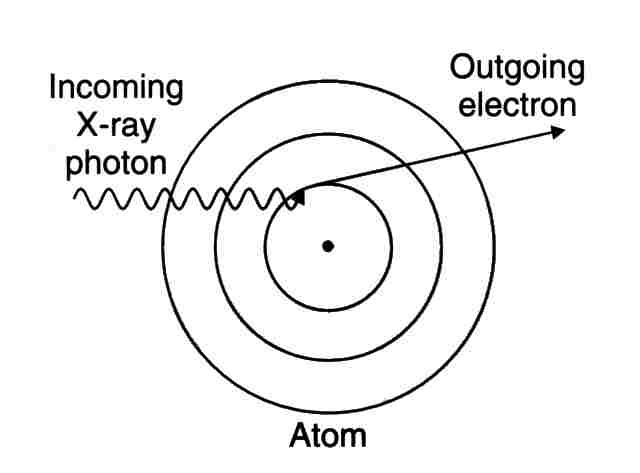
\includegraphics[width=7cm]{../Pictures/Chapter_2/photo_el_2}
\caption[Photo electric effect]{Phenomenology of the photo electric effect}
\label{fig:photo_electric}
\end{figure}
\newpage
\subsection{Compton scattering}

Compton scattering is the inelastic scattering of the incoming photon with a weakly bound electron in the material:
\begin{equation}
\gamma + atom \rightarrow (\gamma ') + e^{-} + atom^{*}
\end{equation}
Contrary to the photoelectric effect, this only concerns quasi-free electrons of the material. 
The photon trasnfers part of its energy to the electron, which is freed from its shell.
Applying conservation of energy and momentum it is possible to derive the energy of the scattered gamma as well as the direction and energy of the freed electron.
\begin{equation}
E_{\gamma '} = \frac{E_{\gamma}}{1+\frac{E_{\gamma}}{m_{e}c^{2}}(1-cos\theta)}
\end{equation}
The angular distribution can be described by the Klein-Nishina formula. It can be noted that forward scattering direction are favoured as the incoming photon energy increases
\begin{equation}
\frac{d\sigma _{cpt}}{d\omega} = Z \cdot \frac{e^{2}}{4\pi \epsilon _{0} m_{e} c^{2}} \cdot \frac{1}{2} \cdot \frac{E'_{\gamma}}{E_{\gamma}} \left( 1 - \frac{E'_{\gamma}}{E_{\gamma}} \cdot sin^{2}\theta + \left[ \frac{E'_{\gamma}}{E_{\gamma}} ^{2} \right] \right)
\end{equation}
The total cross section can be computed by integrating the differential cross section over the angle, with $\epsilon = h\nu / mc^{2}$ and $r_{e} = h/mc$.
\begin{equation}
\sigma _{KN} = 2\pi r_{e}^{2} \left{ \frac{1+\epsilon}{\epsilon ^{2}} \left[ \frac{2(1+\epsilon)}{1 + 2\epsilon} - \frac{ln(1+2\epsilon)}{\epsilon}\right] + \frac{ln(1+2\epsilon)}{2\epsilon}-\frac{1+3\epsilon}{(1+2\epsilon)^{2}}\right]
\end{equation}
\begin{figure}
\centering
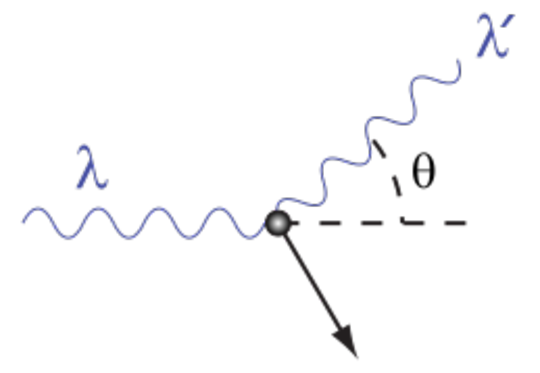
\includegraphics[width=7cm]{../Pictures/Chapter_2/259px-Compton-scattering.pdf}
\caption[Compton scattering]{Phenomenology of Compton scattering}
\label{fig:compton}
\end{figure}

\subsection{Pair production}

If the energy of the gamma exceeds $2m_{e}c^{2} = 1.02$ MeV, the impinging photons can also be converted into an electron-positron pair. The cross-section of the pair production is given at low energies (thus low screening) by
\begin{equation}
\sigma _{pair} = 4\alpha r_{e}^{2} Z^{2} \left( \frac{7}{9}ln2\frac{E}{m_{e}c^{2}} - \frac{109}{54}\right)
\end{equation}
The cross section is very low compared to that of photoelectric and Compton effect until the energy of the $\gamma$ approaches several electron Volts. Thus for the energies involved in medical applications pair production can be neglected.
%\begin{figure}
%\centering
%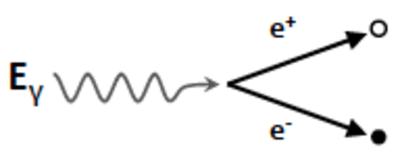
\includegraphics[width=7cm]{../Pictures/Chapter_2/pair_prod.pdf}
%\caption[Pair production]{Phenomenology of pair production}
%\label{fig:pair_prod}
%\end{figure}


\begin{figure}
\centering
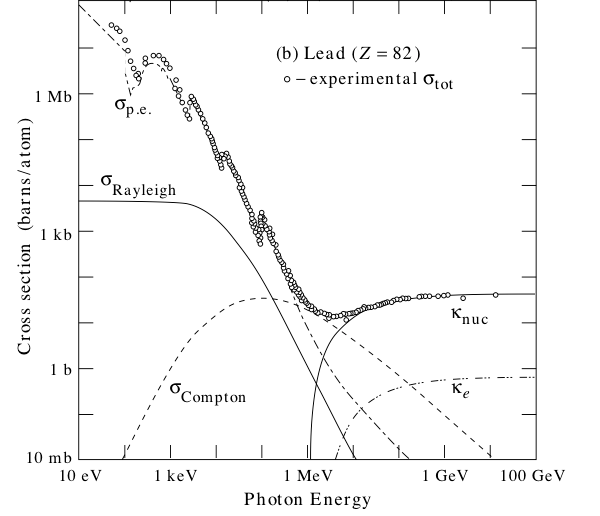
\includegraphics[width=9cm]{../Pictures/Chapter_2/sigma_gamma.pdf}
\caption[$\gamma$ cross section]{Cross section for the different processes in lead}
\label{fig:cross_section}
\end{figure}
\newpage
\section{The scintillation mechanism}

As a general idea the scintillation process can be considered as the conversion of the energy of an incident $\gamma$ quantum or particle into a certain number of low energy photons \cite{Rodnyi1997}. In a way it can be therefore defined as a wavelentgh shifting process \cite{Lecoq2006}.

\begin{figure}
\centering
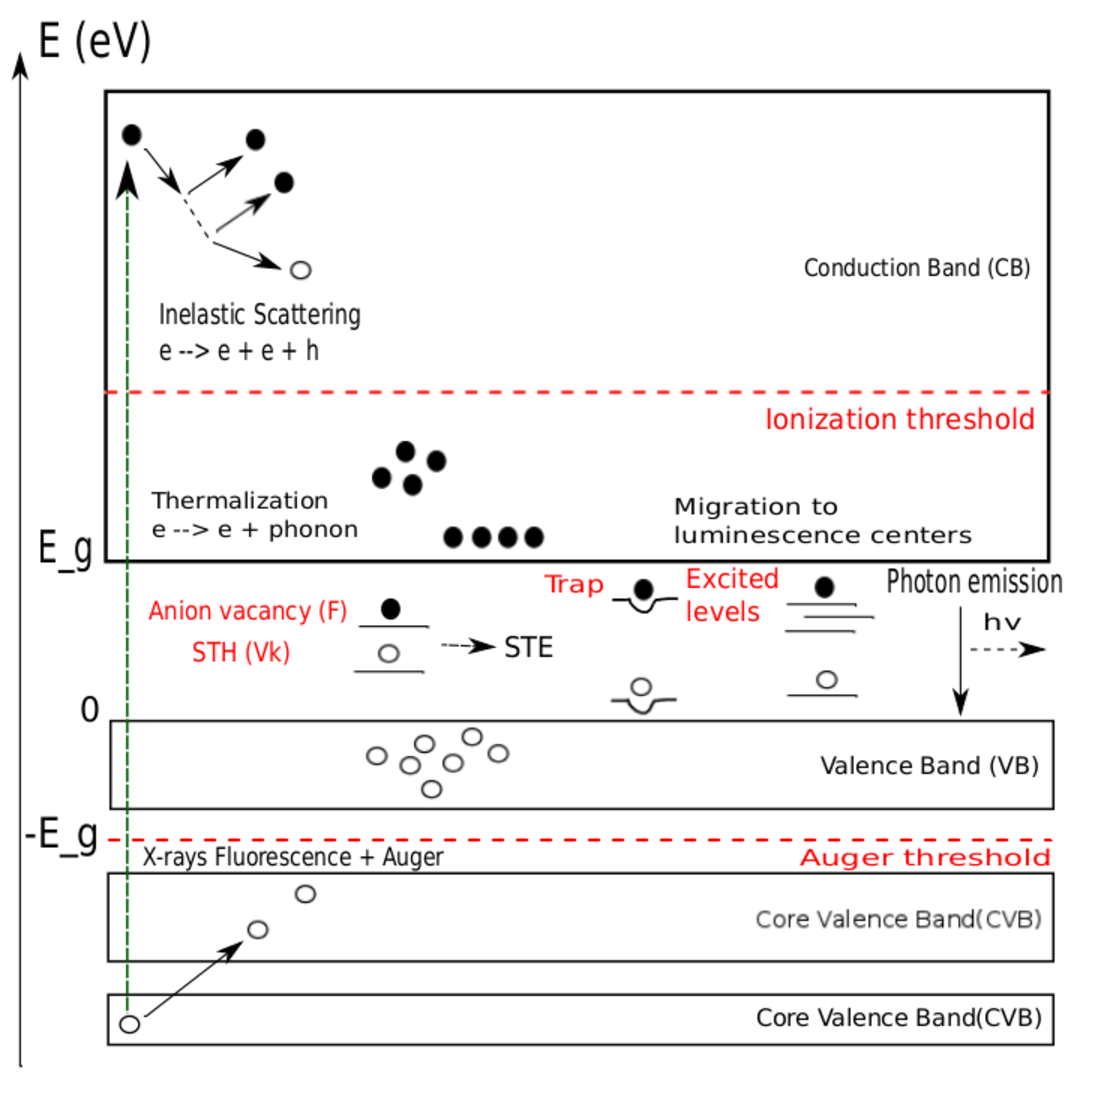
\includegraphics[width=12cm]{../Pictures/Chapter_2/drawing_2.pdf}
\caption[Energy deposition in scintillator]{Chain of energy deposition processes in crystals}
\label{fig:lecoq_easy}
\end{figure}

After a ionization event, generated by the mechanisms presented above in the case of a $\gamma$ interaction, the scintillator relaxes towards a new equilibrium. This process is characterized by a multitude of sub processes, that can be depicted by band diagrams as the one in figure \ref{fig:lecoq_easy}.
As long as the energy of the particles is high enough, it is transferred to secondary particles of low energy, creating an electromagnetic cascade.
A crystal though is an ordered ensemble of atoms, so the electrons in the KeV range start to couple with electrons and atoms of the lattice. As a result of their interaction with electronic states of the material, couples of electrons and relative vacancies are created. The electron hole pairs migrate in the lattice above and below the ionization threshold until they are trapped by a defect or recombine on a luminescent center. Alternatively they cool down by coupling to the lattice vibrations until they reach the top of the valence band (hole) or the bottom of the conduction band (electron). They can also form loosely bound structures called exciton, with en energy slightly smaller than the bandgap energy.
The scintillator itself must contain luminescent centers, either intrinsic or extrinsic (doping ions). These molecular systems in the lattice present characteristic transitions between excited states.
Recombination brings the release of optical photons, at characteristic wavelengths.
%
%The scintillation process can therefore be represented as the sequence of the following stages\cite{Rodnyi1997}: 
%
%\begin{itemize}
%\item Absorption of ionizing radiation and creation of primary e-h pairs
%\item Relaxation of primary e-h pairs with production of secondary e-h pairs, plasmons, photons, etc.
%\item Thermalization of low energy e-h pairs down to the band gap energy $E_{g}$
%\item Energy transfer form the e-h pairs to the luminescence centers
%\item Emission of scintillation photons
%\end{itemize}

\subsection{Creation of electron hole pairs}

To analyze more in depth the mechanisms of the scintillation, we can consider an intermediate energy $\gamma$ ray ( $\sim 500$ KeV) interacting with the scintillator material. In this case the photoelectric effect is dominant. Thus it will produce a hole in a inner shell (usually K shell) and a free or quasifree electron.
\begin{equation}
A + h\nu \rightarrow A^{+} + e
\end{equation}
The energy of the primary electron will be $h\nu - E_{k}$ where $E_{k}$ is the K level energy. The relaxation then happens differently for electrons and holes. 

The ionized atom ($A^{+}$) can relax either radiatively, thus emitting a photon, or nonradiatively, generating a secondary electron. This is know as the Auger effect. Thereafter a cascade of both radiative and nonradiative processes takes place.
The Auger electron and the primary electron begin a proces of electron-electron scattering or phonon emission. In the case of a radiative emission, the soft x-ray photon emitted may be absorbed producing a new deep hole and free electron. 

The electron on the other hand will ionize an atom
\begin{equation}
A + e \rightarrow A^{+} + 2e
\end{equation}
The two undistiguishable electrons will undergo a number of other ionization processes, resulting in an avalanche of secondary electrons and holes. At some point the secondary products of these processes are not able to ionize the medium anymore.
A fast electron can in principle interact also with valence electrons of the medium, producing collective oscillations known as plasmons. Plasmons behave as quasiparticles, with an energy of $\sim 10$ eV and can decay into e-h pairs.

This ensemble of avalanche processes continues until the generated secondaries are not able to create further ionization. At this point electrons and holes start to interact with the vibrations of the lattice in a stage called thermalization, via different mechanisms of electron-phonon interaction. 
 As a consequence, at the end of this chain of de-excitation processes, low energy electronic excitations are present: electrons in the conduction band, holes in the valence band, valence excitons, core excitons.
 
\subsection{Intrinsic luminescence}

\begin{figure}
\centering
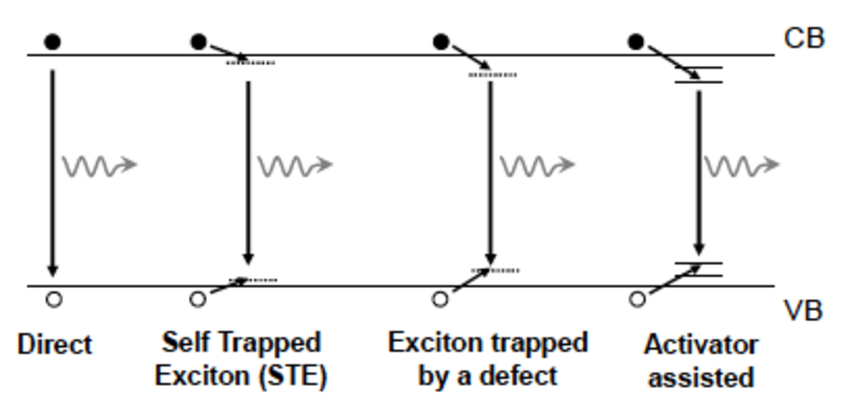
\includegraphics[width=12cm]{../Pictures/Chapter_2/traps.pdf}
\caption[Electron hole recombination]{Different processes for electron hole recombination}
\label{fig:traps}
\end{figure}
Electron and holes have several ways to recombine after thermalization and give rise to scintillation photons.
The simplest emission process is direct recombination
\begin{equation}
e + h \rightarrow h\nu
\end{equation}
Recombination can more effectively take place when the energy of the electron and hole has decreased, so that they form an exciton. 
However the various impurities and lattice defects play a very important role in the scintillation process. Thermalized carriers can be bound in some places of the lattice where atom or defects are localized. 
For example many ionic crystals shows phenomena of localization of the valence hole in the lattice, known as self-trapping. This structure appears when a thermalized hole localizes an anion, polarizing the environment. As a result the hole can be shared between two neighbouring ions forming a $V_{k}$ center, and the hole is defined as self-trapped hole. For high energy excitation direct creation of valence exciton is unlikely, so $V_{k}$ centers usually capture free electrons. From subsequent de excitation they can emit photons, thus giving rise to the excitonic luminescence.
\begin{equation} 
e + h \rightarrow ex \rightarrow h\nu
\end{equation}

\subsection{Core to valence transitions}

If the core bands of the scintillator lie below the Ager threshold, the most favoured transitions involve holes in the valence band and electron in the conduction band. Some systems though present the so-called cross luminescence. This phenomenon implies a direct core to valence transition, due to the fact that holes in uppermost core bands can not de excite non radiatively \cite{Lecoq2006}. 

A notable example of core to valence transition is $BaF_{2}$. In this system a $Ba^{2+}$ $5p$ core hole is above the Auger threshold and hence Auger effect does not occur. They can recombine directly with electrons from the valence band, in most of the cases radiatively.
This leads to a very fast luminescence given by recombination of the core hole, while the primary electron de excitation is more complex thus leading to a slower component.

\begin{figure}
\centering
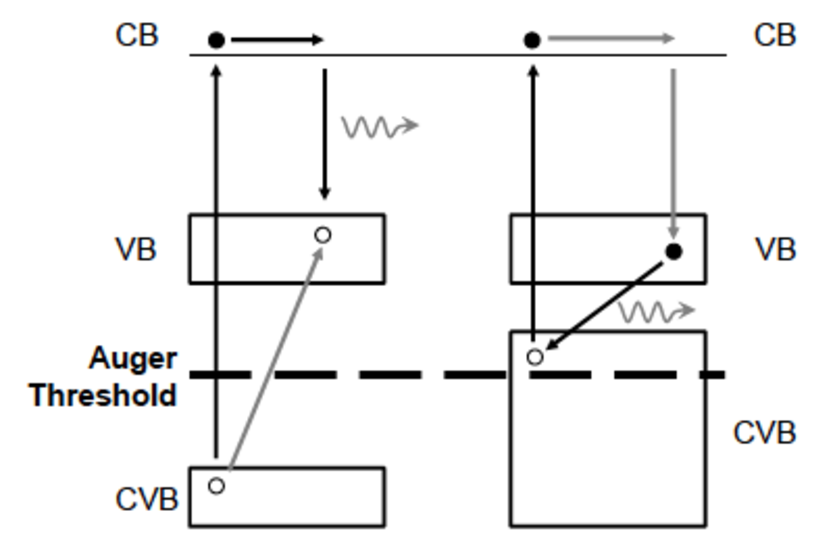
\includegraphics[width=8cm]{../Pictures/Chapter_2/core_to_valence.pdf}
\caption[Core to valence luminescence]{Direct luminescence (left) versus cross to valence luminescence (right)}
\label{fig:CTV}
\end{figure}
 

\subsection{Extrinsic luminescence}

Most of the scintillator samples used in this work are extrinsic, that is doped with activation centers that can enhance the intrinsic scintillation properties presented above by favouring direct recombination.
Rare earth ions doping, for example, is largely used in scintillator technology because of the parity and spin-allowed transition $4f^{n-1}5d\rightarrow 4f^{n}$. 
Extrinsic scintillators usually present different luminscent mechanisms driven by activated sites \cite{Lecoq2006}:
\begin{itemize}
\item $e + h + A \rightarrow ex + A \rightarrow A^{*} \rightarrow A + h\nu$
\item $e + h + A \rightarrow A^{1+} + e \rightarrow A^{*} \rightarrow A + h\nu$
\item $e + h + A \rightarrow (A^{1-})^{*} + h \rightarrow A + h\nu$
\item $A \rightarrow A^{*} \rightarrow A + h\nu$
\end{itemize}
In the first case the insertion of dopants is able to sufficiently quench the exciton luminescence so that excitation of radiative centers results form a transfer from excited matrix states.
A competing process is the direct capture of free thermalized carriers by luminescent center, in the case of electrons or holes.
In heavy doped or self-activated crystals ($CeF_{3}$) direct excitation by ionizing radiation is possible.

%QUI MANCA QUALCOSA!

\subsection{Quenching phenomena}
TO DO
% thermal, concentration, trapping Chapter3 Lecoq
\section{Operational parameters}
\subsection{Light yield}
One of the feature commonly required of a scintillator is to have a high light yield, that is to be an efficient converter of radiation to visible light.
In this case the relative light output of the scintillator, $L_{R}$, can be considered the significant quantity. It is defined as the number of emitted photons per unit of absorbed energy \cite{Rodnyi1997}
\begin{equation}
L_{R} = \frac{N_{ph}}{E_{\gamma}}
\end{equation}
The number of produced e-h pairs $N_{eh}$ depends on the average energy needed for the creation of a low energy e-h pair, $\chi _{eh}$. This value depends on the type of lattice and band gap of the material, with a numerical coefficient $\beta$
\begin{equation}
\chi _{eh} = \beta \cdot  E_{g}
\end{equation}
If $\alpha$ is the average number of scintillation photons produced by a single e-h pair, the light output is
\begin{equation}
L_{r} = \frac{\alpha \cdot N_{eh}}{E_{\gamma}} = \frac{\alpha}{\chi _{eh}} = \frac{\alpha}{\beta \cdot E_{g}}
\end{equation}
The coefficient $\alpha$ depends on the transport efficiency of the e-h pairs to the luminescence center and the conversion efficiency of the center itself.

\subsection{Optical properties and light transport}
% MANCA QUALCOSA!
TO DO
\subsection{Energy resolution and nonproportionality}
In the case of $\gamma$ spectroscopy it is necessary to discriminate quanta with different energy.
For scintillation detector this fundamental property is characterized by the energy resolution $R$, defined as $\Delta E/E$ (in $\%$) where $\Delta E$ is the full width at half maximum (FWHM) at pulse height $E$.
It depends on the characteristics of the scintillator, i.e. materials, size and defects as well as the coupling with the photo detector and the parameters of the photo detectors itself. Statistical fluctuations at any step of the detector chain, from dynode multiplication to photo cathode efficiency in the case of a PMT can worsen the resolution at the peak. 
Thus energy resolution can be defined as \cite{Rodnyi1997}
\begin{equation}
R^{2} = R_{S}^{2} + R_{PM}^{2} = R_{S}^{2} + \frac{\delta}{E_{\gamma}}
\end{equation}
where $R_{S}$ and $R_{PM}$ are, respectively, the scintillator and photomultiplier contributions and $\delta$ includes photo electron statistics.
It is possible to further decompose the scintillator resolution $R_{S}$ to take into account the factors depending on the type of scintillator used. In particular it is useful to introduce a term for the transfer efficiency of the optical photons $R_{S}$, a term for inhomogeneity $R_{i}$ and a term for nonproportionality $R_{n}$
\begin{equation}
R_{S}^{2} = R_{t}^{2} + R_{i}^{2} + R_{n}^{2}
\end{equation}
The interest lies in the fact that the two terms, for inhomogeneity and nonproportionality, account for the intrinsic resolution of the crystal.
Inhomogeneity arise from possible imperfections of the scintillator, such as local variations in the concentration of the dopant or optical defects.

Non proportionality arise when scintillators show deviation from stability of excitation spectrum, that is when linearity between energy of the excitation and relative light output is not preserved. This is particularly important for low energy excitation, since scintillation phenomena occur mainly on the surface. Non proportionality is caused by the statistical nature of the creation of secondary electrons and photons and contribute to worsen the resolution.

\subsection{Cerenkov effect}
Cerenkov radiation brings important information both in high energy physics and time resolved PET.
Cerenkov radiation occurs when a charged particle passes through a dieletric medium at a speed greater than the phase velocity of light in that medium.
The phase velocity of light in a medium of refractive index $n > 1$ is
\begin{equation}
v_{p} = \frac{c}{n}
\end{equation}
A charged particle can travel faster than the speed of light if, given its velocity $v_{p}$ 
\begin{equation}
\frac{c}{n} < v_{p} < c
\end{equation}
This translates to the following condition for the $\beta$ coefficient of the particle
\begin{equation}
\beta = \frac{v_{p}}{c} > \frac{1}{n}
\end{equation}
For a particle of a given mass thus the energy threshold is
\begin{equation}
K_{thr} = mc^{2}\left( \frac{\sqrt {n^{2}-1}}{n} - 1 \right)
\label{eq:thr}
\end{equation}
The phenomenology of Cerenkov effect can be explained considering the polarization of the medium caused by a charged particle trasversing it.
Below the Cerenkov threshold the dipoles sorrounding are simmetrically arranged around the path. As the particle crosses the threshold it travels faster the the speed at which it interacts with the dipoles. This simmetry breaking leads to a non-vanishing dipole moment and thus to the formation of a wave front.

\begin{figure}
\centering
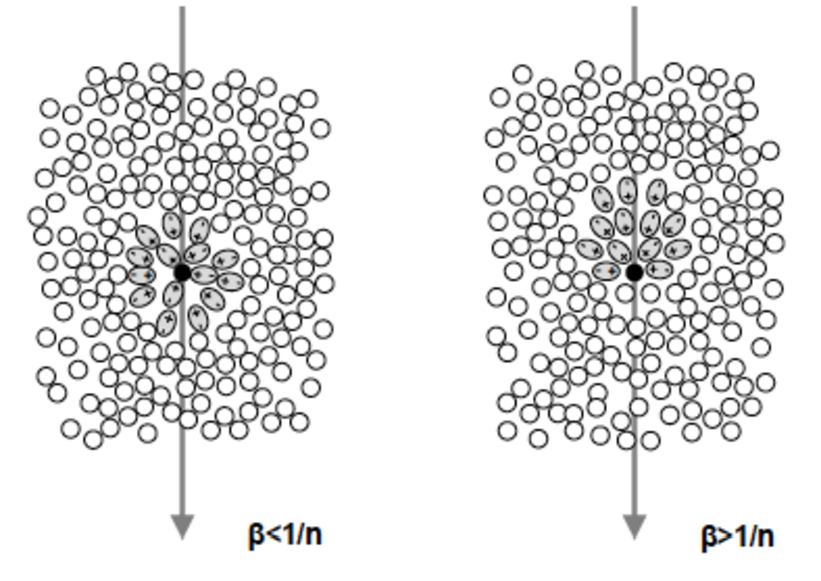
\includegraphics[width=9cm]{../Pictures/Chapter_2/cerenkov.pdf}
\caption[Cerenkov effect]{Phenomenology of Cerenkov effect}
\label{fig:cerenkov}
\end{figure}

Cerenkov photons are emitted at a characteristic angle in the forward direction, obtained via simple geometrical considerations. The distance traveled by the charged particle in a time $t$ is $t\cdot \beta \cdot c$ whereas the distance along which the photon propagates is $t\cdot c /n$ as shown in figure \ref{fig:cone}.
Therefore the characteristic angle at which photons are emitted can be calculated as
\begin{equation}
cos(\theta _{C}) = \frac{t c/n}{t \beta c} = \frac{1}{n\beta}
\end{equation}
As will be shown in the next chapter, the direction of emission retains a primary interest in the field of particle identification, while it has a negligible impact on timing measurement in PET scanners. It is worth to be noted though that the Cerenkov photons are emitted promptly, taking a relevant share of the first incoming photons.  
\begin{figure}
\centering
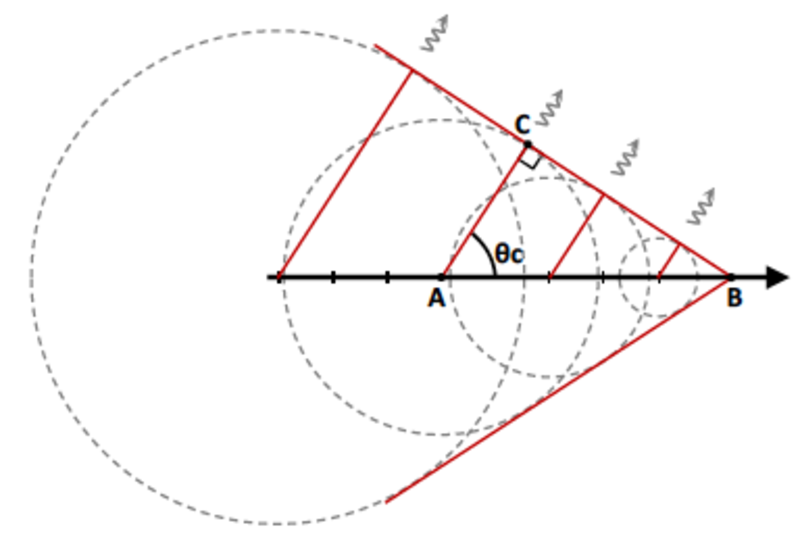
\includegraphics[width=9cm]{../Pictures/Chapter_2/cone.pdf}
\caption[Cerenkov emission cone]{Sketch of the Cerenkvo emission cone}
\label{fig:cone}
\end{figure}
It is useful to consider the number of emitted photons per unit length by a charged particle as a function of the wavelength
\begin{equation}
\frac{dN}{d\lambda dx} = \frac{2\pi z^{2}\alpha}{\lambda ^{2}}\left( 1 - \frac{1}{\beta ^{2}n^{2}(\lambda)} \right)
\end{equation}
Neglecting dispersion in the medium, and integrating over an appropriate interval of waveleghts we obtain that the photons are emitted mostly in the UV range.
\begin{equation}
\frac{dN}{dx} = 2\pi z^{2} \alpha \left( 1-\frac{1}{\beta ^{2} n^{2} (\lambda)}\right) \int _{\lambda _{1}} ^{\lambda _{2}} \frac{d\lambda}{\lambda ^{2}}  = 2\pi z^{2}\alpha sin^{2}\theta _{C} \left( \frac{1}{\lambda _{1}}-\frac{1}{\lambda _{2}}\right)
\label{eq:number}
\end{equation}

A simple calculation shows that, even at the low energies that characterize a PET exam (511 KeV), a non negligible number of Cerenkov photons is produced.
As an example, it is interesting to consider the case of the most popoluar crystal for PET detectors, Lu$_{2}$SiO$_{5}$:Ce (LSO) with a density $\rho _{LSO}$ = 7.48 g/cm$^{3}$ and a refractive index of 1.82 \cite{jellison2012}.
Given the K-shell binding energy of the electron (63 KeV \cite{xdata2009}), we can estimate, with the help of formula  \ref{eq:thr}, the energy threshold for Cerenkov production for electrons at 448 KeV.
If we then consider a freed electron from the K-shell and its average range in LSO (265 $\mu$m \cite{nist2005}), we can make use of formula \ref{eq:number}, given that
\begin{equation}
sin ^{2}(\theta _{c}) = 1 - \frac{1}{n^{2}\beta ^{2}} = 0.58
\end{equation}
The number of optical photons produced in the wavelength range 180 - 800 nm is $\sim$ 40.


\section{Scintillation processes in the samples analyzed}
TO DO
% e invece qui approfondiamo i sample nostri
% magari puoi anticipare due cose sulle terre rare

\subsection{Lutetium Ortho Silicate}

\subsection{Lutetium Aluminum Garnet}

\subsection{Cerium Fluoride}

\subsection{Bismuth Germanate}} % A regular chapter, starts with '\chapter{Title}'
% citazioni, immagini

\chapter{Photo detectors}
During the scintillation phase visible photons are generated and coupled to a photo detector. At this stage the photo detector generates an electric signal related to the photon rate, by generating free electrons in vacuum or electron-hole pairs in a semiconductor.

As they are used as fundamental components of the experimental apparatus, the vacuum photo detector technology and the solid state technology will be presented.
Vacuum photo detectors are characterized by the production of free electrons in an external photo cathode by photoelectric interaction. The produced electrons undergo acceleration in a focused electric field and are multiplied by secondary interaction before being transferred to the read out circuitry. Photo multiplier tubes (PMT) and micro channel plates tubes  (MCP-PMT) are prominent examples of vacuum technology.
  
In the case of solid state photo detectors, photons interact directly in the bulk material, where electron-hole pairs are produced. The pairs are then accelerated in the electric field and multiplied by ionization in the semiconductor itself. In the work presented here, Silicon photo multipliers (SiPM) are used as representative of this kind of detector.     

\section{Photo multiplier tubes}

Photo multiplier tubes are largely used vacuum photo detection devices and have been thoroughly discussed in literature \cite{Knoll2000}. 
\begin{figure}[htbp]
\begin{center}
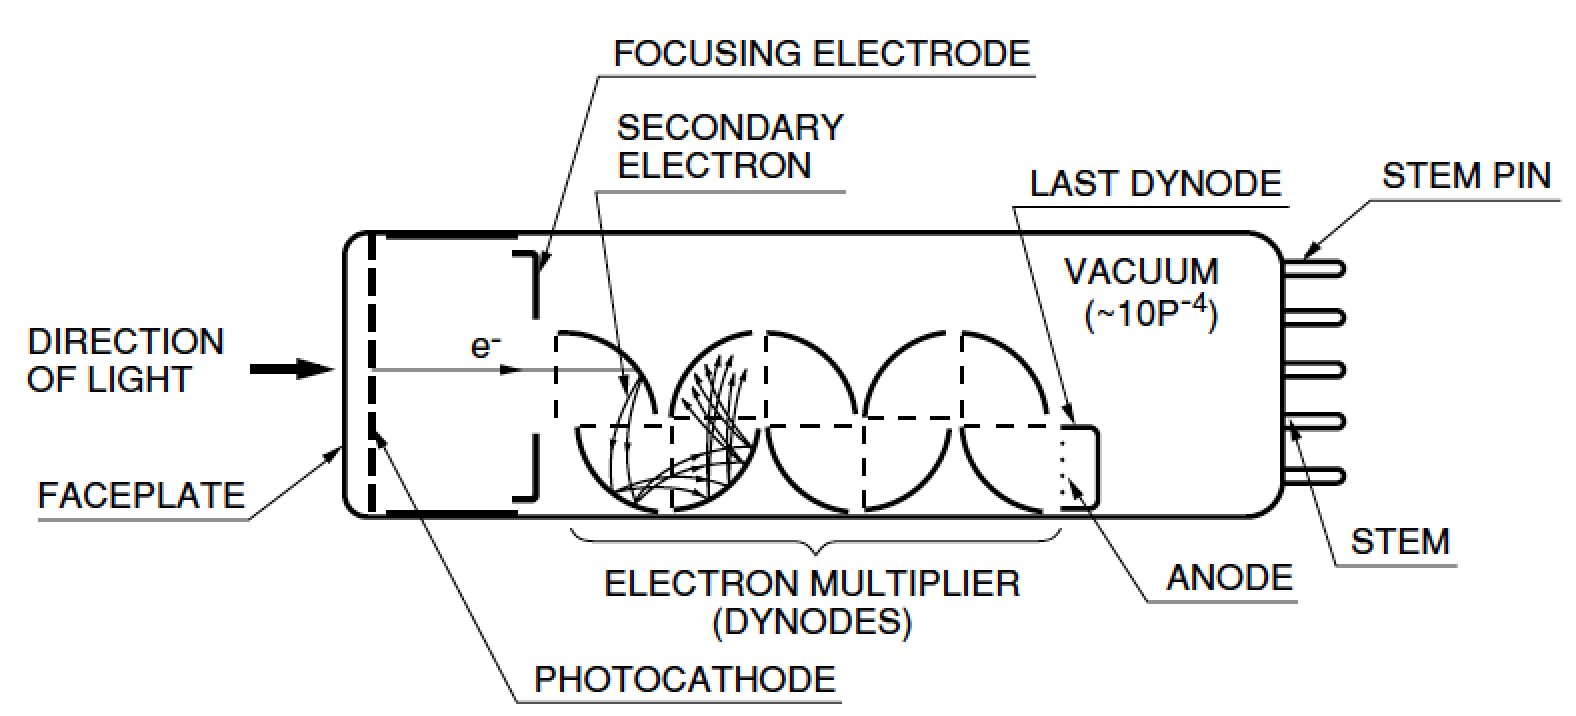
\includegraphics[width=12cm]{../Pictures/Chapter_3/PMT.png}
\end{center}
\caption[PMT schematics]{Schematics of a Photo-Multiplier Tube \cite{Hama2006}.}
\label{fig:PMT_schematics}
\end{figure}

In figure \ref{fig:PMT_schematics} the main elements of a photo multiplier tube are sketched:
\begin{itemize}
\item a photocathode, which converts visible photons into an electron flux
\item an electron-optical input system which focuses and accelerates the electron flux
\item an electron multiplier consisting of a series of secondary emission electrodes (dynodes)
\item an anode, which collects the electron flux and supplies the output signal
\end{itemize}
Photoemission is due to a fraction of the incident visible photons that transfer enough energy to the electrons of the photo cathode to extract them.
Then the focusing system allows the freed electrons to reach the first dynode, i.e. the first multiplication stage. The electrons are accelerated and focused by electric field between the dynodes and the required potential gradient is usually guaranteed by a voltage divider.

%foto divider

\subsection{Properties of PMT}
\begin{itemize}
\item \textbf{quantum efficiency}: photo cathode are usually made of deposited photo emissive semiconductor. They can be semi transparent or opaque, depending on the place where the emissive material is deposited with respect to the input window.
The most used materials are silver-oxygen-caesium (AgOCs), Antimonyum Caesium (SbCs), and the bi-and trialkali compounds SbKCs, SbRbCs, and SbNa$_{2}$KCs. The most important parameter to be considered is the cathode radiant sensitivity, defined as the ratio of the cathode current $I_{p}$ to the incident flux $\Phi$
\begin{equation}
S_{k}(A/W)=\frac{I_{p}(A)}{\Phi _{e}(W)}
\end{equation}
The incoming photons have usually a certain spectral composition and the cathode is not uniformly sensitive in this range. With this respect the most used quantity is the quantum efficiency, that is the ratio of the number of photo electrons emitted, $n_{k}$, to the number of incident photons, $n_{i}$
\begin{equation}
QE = \frac{n_{k}}{n_{i}} = S_{k, \lambda} \frac{h\nu}{e}
\end{equation}
where $e$ is the electron charge and $S_{k, \lambda}$ is the monochromatic sensitivity, defined as
\begin{equation}
S_{k, \lambda} = \lim_{d\lambda \to 0}\frac{dI_{p}}{d\Phi _{e}}
\end{equation}
%foto QE
\item \textbf{gain}: if the number of photo electrons that reach the first dynode is $n$, and the gain of the dynode is $g_{1}$, the number of secondary electrons is $n\cdot g_{1}$. If $g_{i}$ is the gain of the single dynodes, after $N$ stage the number of electrons collected at the anode are
\begin{equation}
n_{a} = n\prod_{i=1}^N g_i
\end{equation}
It is possible to define the gain of the photo multiplier as the ratio $I_{a}/I_{p}$ where $I_{a}$ is the anode current given by a photo current $I_{p}$. If we define a collection efficiency for each dynode, depending of geometrical parameters, $\eta _{i}$, then the gain $G$ is
\begin{equation}
G = \eta \prod_{i=1}^N \delta _{i} \eta _{i} = \eta \prod_{i=1}^N g_{i}
\end{equation}
Typical gains can go up to 10$^{9}$.
\item \textbf{transit time spread}: transit time spread is the transit-time fluctuation of the signal when identical light pulses hit the same part of the photo cathode. The time resolution of a tube is then often quoted as the FWHM of the probability distribution of the fluctuations.
If the probability distribution of electrons arriving at the anode is assumed to be Gaussian, then the response $R_{\delta}(t)$ to a delta-function light pulse is
\begin{equation}
R_{\delta}(t) = \frac{1}{\sigma _{R}\sqrt {2\pi}}\exp{\left( -\frac{(t-t_{tts})^2}{2\sigma _{R}^2}\right)}
\end{equation}
where $t_{tts}$ is the mean transit time.
\end{itemize}

\section{Micro Channel Plate-PMT}
\begin{figure}[htbp]
\begin{center}
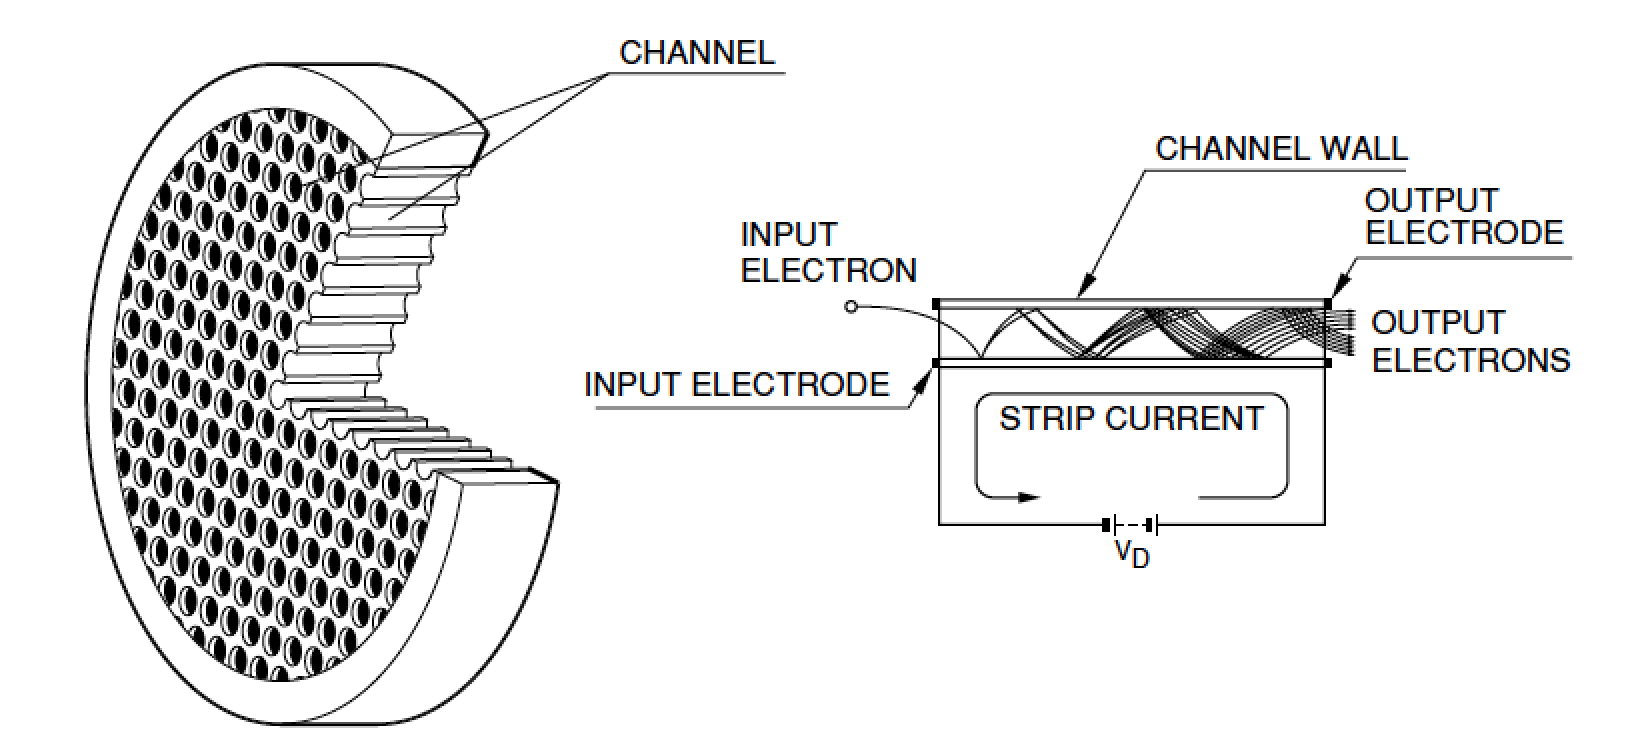
\includegraphics[width=12cm]{../Pictures/Chapter_3/MCP_plate.png}
\end{center}
\caption[MCP principle]{Work principle of a Micro Channel Plate \cite{Hama2006}.}
\label{fig:MCP_schematics}
\end{figure}
A micro channel plate is a two-dimensional array of glass capillaries mounted in parallel as shown in figure \ref{fig:MCP_schematics}.
The diameter of the channels lies in a range of 5 to 20 microns and their internal walls are treated so to have a defined electrical resistance and secondary emissive properties.
At both ends of the plate high voltage is applied, so that a primary electron impinging on the wall of a channel produces a multiplication chain.
Since they resemble in function a structure of dynodes, microchannel plates are usually used in combination with vacuum detector technology in an assembly known as MCP-PMT, as shown in figure \ref{fig:MCP_struct}.

A MCP-PMT consists of an entry window, a photo cathode, one or more micro channel plates and a collecting anode.
To operate a MCP-PMT it is necessary to provide a certain voltage to the system. To this purpose standard voltage divider circuits are usually adopted, in order to guarantee drifting spaces for electrons before and after the photo cathode, and multiplication in the MCP stack \cite{Hama2006}.
%divider  

  
\subsection{Properties of MCP}
\begin{figure}[htbp]
\begin{center}
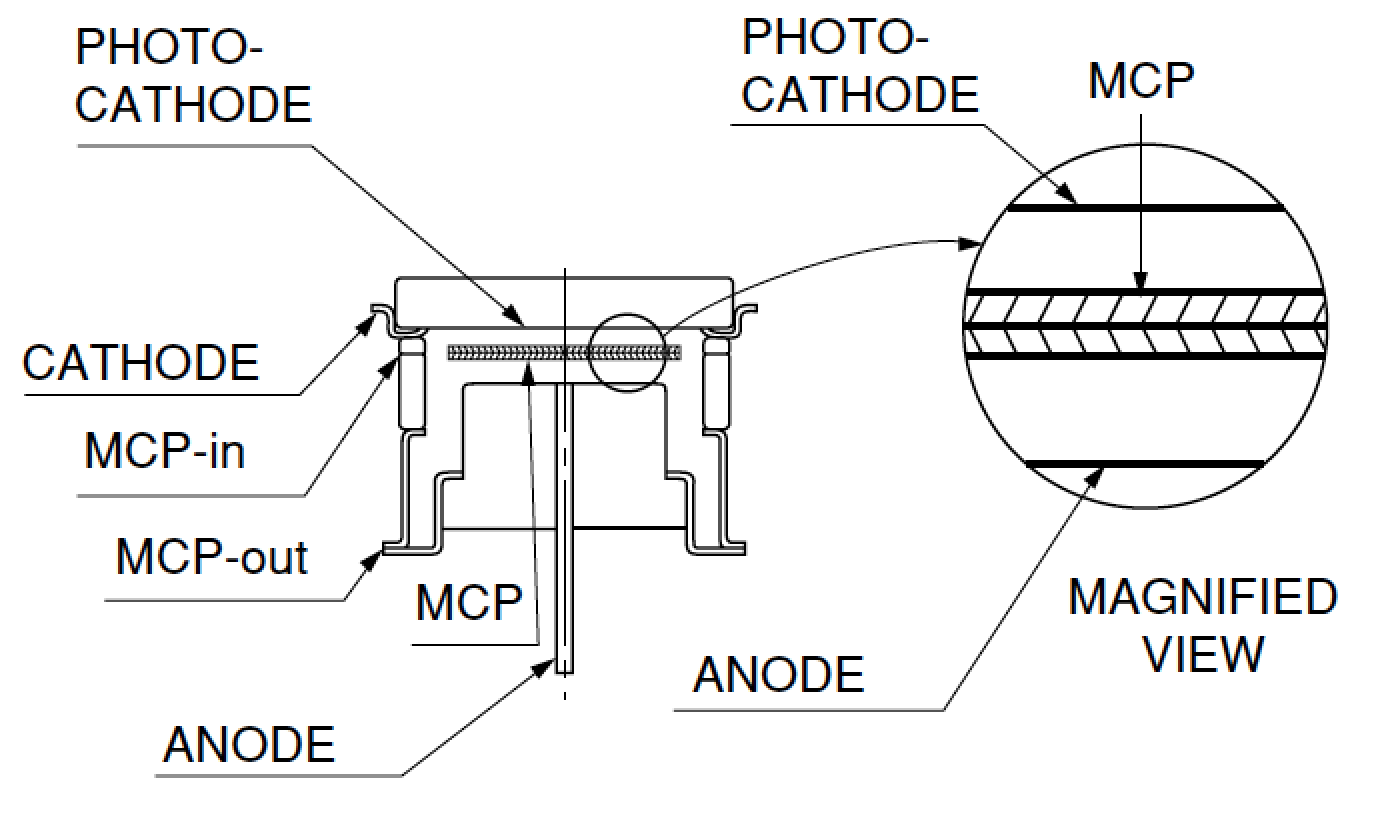
\includegraphics[width=12cm]{../Pictures/Chapter_3/MCP_struct}
\end{center}
\caption[MCP schematics]{Schematics of a MCP-PMT \cite{Hama2006}.}
\label{fig:MCP_struct}
\end{figure}
\begin{itemize}
\item \textbf{quantum efficiency}: in terms of quantum efficiency they do not differ from standard PMTs, since they use of the same photo cathode technology.
\item \textbf{gain}: the gain of an MCP-PMT depends primarily on the number of plates stacked. Geometrically is determined by the length-to-diameter ratio af a channel $\alpha$, as
\begin{equation}
G = \exp{\left( \frac{\Delta \cdot L}{d} \right)} = \exp{\left( \Delta \cdot \alpha \right)}
\end{equation}
where $\Delta$ is the gain factor and depends on the plate material, $L$ and $d$ are, respectively, the length and diameter of the micro tube.
Typical gains range from 10$^{4}$ to 10$^{6}$.
%gain curve
\item \textbf{ion feedback, electron back scattering}: strongly correlated with the characteristics of gain are the problems of ion-feedback and electron back scattering. As the voltage, and thus the gain, increases, it is more and more likely for a photo electron to be back scattered towards the photo cathode or for an ion to undergo the same process from the stack. Ions can be commonly stripped from residual gas in the drifting area or from interaction in the plate.
This leads to the production of secondary pulses, that contribute to the worsening of the time response of the device.

Connected to this is also the issue of ageing, since ion bombardment damages the photo cathode as the vacuum in the device degrades with time.
Partial solution to this problem has been found by depositing an Aluminium protection layer on the plate and by modifying the inclination of the micro tubes in the so called Chevron geometry \cite{Vavra2004}.
%immagine su ion feedback

\item \textbf{time characteristics}: the rise and fall time of a MCP-PMT are ultra-short, due to the multiplication characteristics of the device. This translated into typical signals contained in a few ns, or even less. For timing application the most important parameter to consider is the transit time spread (TTS). The TTS is the spread in the arrival time of a bunch of photon produced by a converted electron in the photo cathode. The time response of MCP-PMTs will be analysed further in the next chapters.

%typical IRF
\end{itemize}

\section{Silicon photo multipliers}
Recently solid state photo detectors have become competitive with vacuum devices, and for some applications they represent the ideal solution. Their advantage lies in the high photon detection efficiency, their low sensitivity to high magnetic fields, their compactness and cost efficiency \cite{Dolgoshein2003}.
In particular the insensitivity to high magnetic fields, given by the feature that no electrons are travelling in the vacuum between dynode and dynode, makes the solid photo detector the first choice for PET-MRI scanners or high energy experiments. With respect to the MCP-PMT, also characterized by high operability in magnetic fields, silicon devices still maintain a high photon detection efficiency, that is the conversion efficiency of incoming photons into electron hole pairs determining in principle a better energy and time resolution.
\begin{figure}[htbp]
\begin{center}
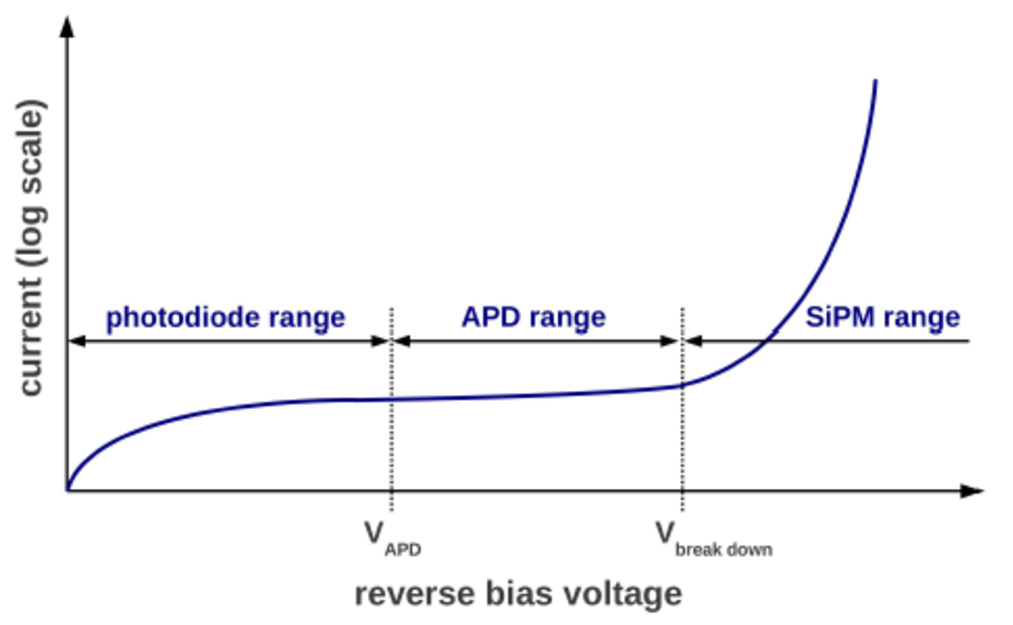
\includegraphics[width=12cm]{../Pictures/Chapter_3/avalanche.pdf}
\end{center}
\caption[I-V plot Silicon detectors]{Voltage current plot for Silicon devices. SiPMs work in Geiger mode \cite{Gundacker2014}.}
\label{fig:avalanche}
\end{figure}

Solid state photo detectors are usually p-n junctions reversely biased and, depending on the value of the bias voltage, different operational parameters adapt to fundamentally three modes.
As seen in figure \ref{fig:avalanche} the voltage can applied can be low, as in photo diodes, leading to low currents proportional to the incoming flux. Moving towards the proportionality region the freed electrons are able to ionize further, thus determining a net gain of the device. Avalanche photo diodes (APDs) are a common device operated in this region.
Finally a third region, characterized by non-proportionality is the operating segment of Geiger mode APD (G-APD). In the Geiger mode region both electrons and holes are able to further ionize the bulk, and the device is sensible to single photo electrons. The created avalanche must be quenched either externally by a series of quenching resistors or actively.
Many G-APD cells connected in parallel are the basic structure of silicon photo-multipliers (SiPM) or multi pixel photon counters (MPPC).

\begin{figure}[htbp]
\centering
\begin{subfigure}
  {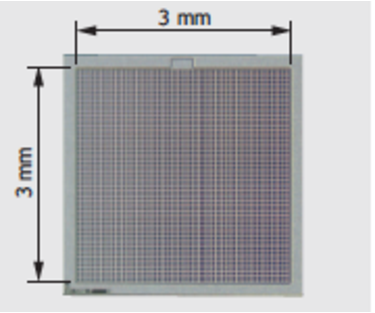
\includegraphics[width=6cm]{Pictures/Chapter_3/mppc_photo.pdf}}
\end{subfigure}
\begin{subfigure}
  {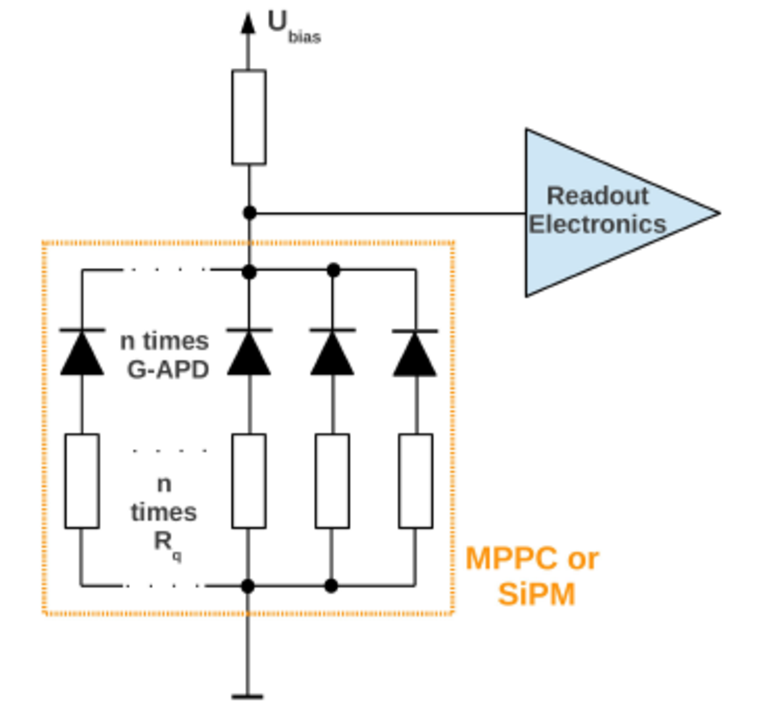
\includegraphics[width=6cm]{Pictures/Chapter_3/mppc_schema.pdf}}
\end{subfigure}
\caption[Example of SiPM]{Example of Hamamatsu MPPC (left) and basic strucutre of a SiPM (right) \cite{Gundacker2014}.}
\label{fig:mppc}
\end{figure}

\subsection{Analog SiPM}
The structure of an analog SiPM is composed by series of Geiger mode cells in parallel, and the self sustained avalanche is usually quenched by external resistors or active quenching circuitry. The basic schema of a standard SiPM with quenching resistors is shown in figure \ref{fig:mppc}.

The structure of a G-APD optimized for detection of blue light is shown in figure \ref{fig:uvir}.
On top of the low resistivity bulk layer an epitaxial layer with a high dopant concentration region is located.
The implantation of opposite charge constitutes the p-n junction with a very thin layer extremely doped to assure electric field uniformity.
The cell and the quenching resistor are connected on the top surface.
Finally a passivation layer (SiO$_{2}$) protects the device. Due to its low index of refraction (n $=1.55$ in the blue) with respect to the one of Silicon (n$=3.5$) Fresnel losses can occur, usually compensated by the presence of anti-reflection coatings.
\newpage
\begin{figure}[htbp]
\centering
\begin{subfigure}
  {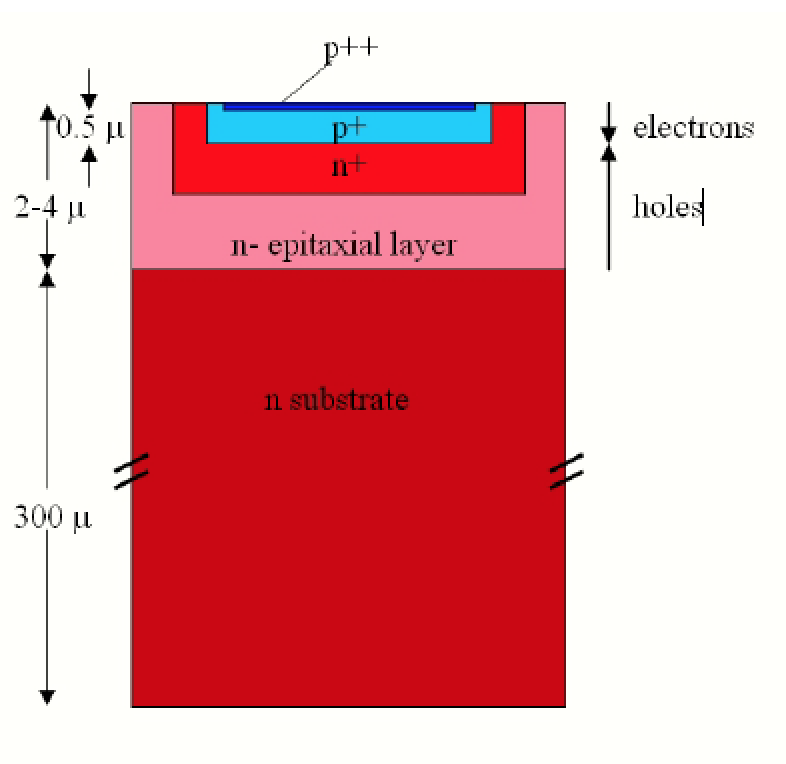
\includegraphics[width=6cm]{Pictures/Chapter_3/IR_mppc}}
\end{subfigure}
\begin{subfigure}
  {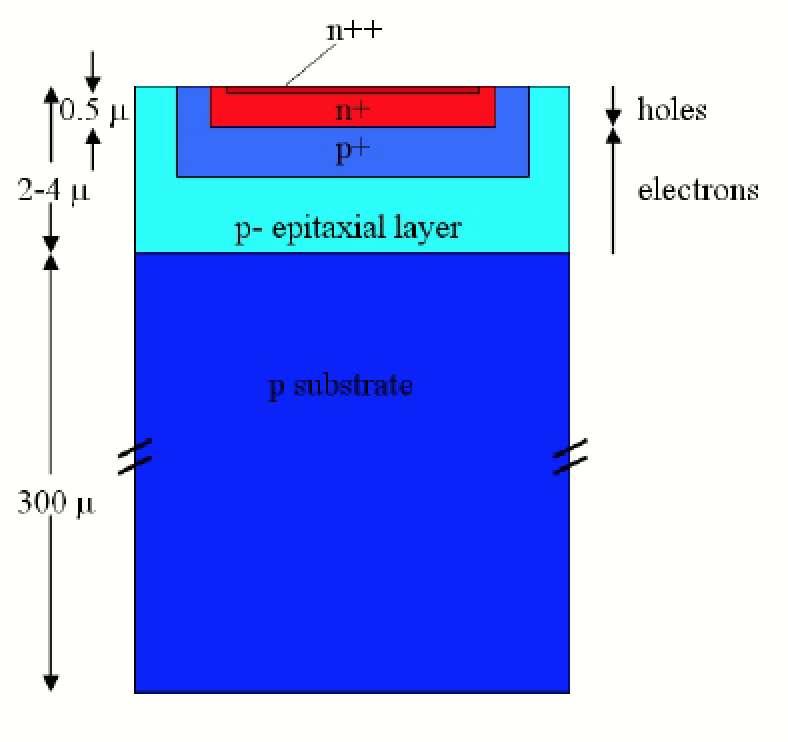
\includegraphics[width=6cm]{Pictures/Chapter_3/UV_mppc}}
\end{subfigure}
\caption[SiPM layer structure]{Layered structure of a IR (left) and UV (right) SiPM \cite{Gundacker2014}.}
\label{fig:uvir}
\end{figure}

\subsection{Properties of SiPM}
\begin{itemize}
\item \textbf{photon detection efficiency}: the photon detection efficiency can be defined as
\begin{equation}
PDE = QE \cdot \epsilon \cdot P_{avalanche}
\end{equation}
where $QE$ is the quantum efficiency, $\epsilon$ is the geometric fill factor and $P_{avalanche}$ is the probability of triggering an avalanche.
The $QE$ has already been introduced for ordinary photo cathodes and it is comprehensive of Fresnel losses.
The fill factor $\epsilon$ is defined as the ratio of the sensitive area to the total area of the detector.
Finally the $P_{avalanche}$ is the probability of an electron or hole to cause an avalanche and it depends on the bias over voltage.
% tipical value

\item \textbf{gain}: the gain of an analog SiPM can be written as
\begin{equation}
G = \frac{C\cdot U_{ov}}{q}
\end{equation}
where $C$ is the cell capacitance, $U_{ov}$ is the bias over voltage and $q$ is the charge $q = 1.602 \cdot 10^{-19} C$.
This value is typically between $10^{5}$ and $10^{7}$.

\item \textbf{spurious events} a dark count is the random production of charge carriers in the depleted region which leads to a regular signal. This type of unwanted event is typically uncorrelated, provided the the dark count rate (DCR) is low enough. It strongly depends of temperature, and typical values range between $100$ kHz to few MHz at $25^{\circ}$C.

Optical crosstalk on the other hand is determined by the trigger of an avalanche by an optical photon produced in a neighbouring cell. Indeed optical photons produced in avalanches can travel to other cells, causing correlated spurious pulses. These pulses can occur even after a delay of several $\mu$s, due to the secondary photons generating electron hole pairs.

Moreover charge carriers can be trapped in the bulk and released tens to hundreds of ns later determining after pulsing.

\item \textbf{saturation}: if SiPMs are exposed to high photon fluxes, saturation effects may occur. The detector is intrinsically limited by the number of cells: if the number of photons is small compared to the number of cells provided PDE correction, the SiPM signal is proportional to the light signal. In the opposite case, the signal is saturated.
\end{itemize}

\subsection{The NINO chip}
Signal generated by SiPMs are in the range of mV, thus we make use of low noise electronics to read out the detector. In the study presented the ultra fast front-end preamplifier-discriminator chip called NINO, developed at CERN \cite{Anghinolfi2004}, has been chosen. Originally designed for the time-of-flight sub detector of the ALICE experiment, it matches the main requirements of a SiPM readout, that is speed, low noise, minimum slew rate, low input impedance.
\begin{figure}[htbp]
\begin{center}
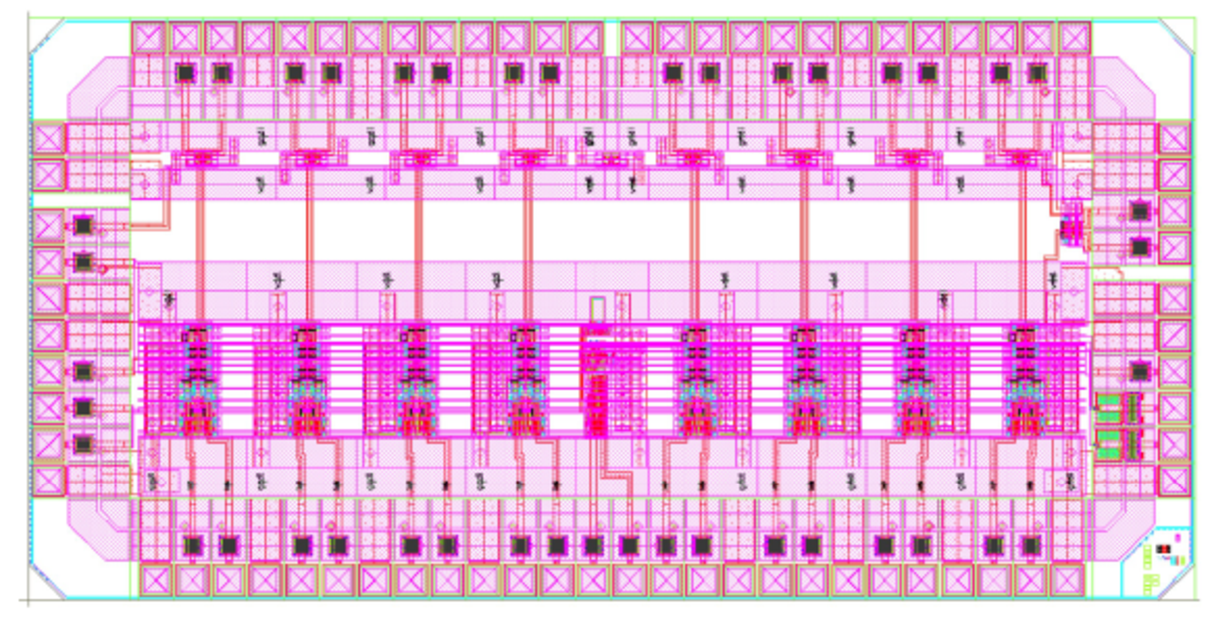
\includegraphics[width=9cm]{Pictures/Chapter_3/NINO.pdf}
\end{center}
\caption[Scheme of the NINO chip]{Scheme of the NINO chip.}
\label{fig:nino_foto}
\end{figure}

The chip has eight channels, designed for differential readout. Each channel is characterized by an amplifier with 1-ns peaking time, a discriminator with a minimum detection threshold of 10 fC and an output stage. The scheme of the chip is shown in figure \ref{fig:nino_foto}.
\begin{figure}[htbp]
\begin{center}
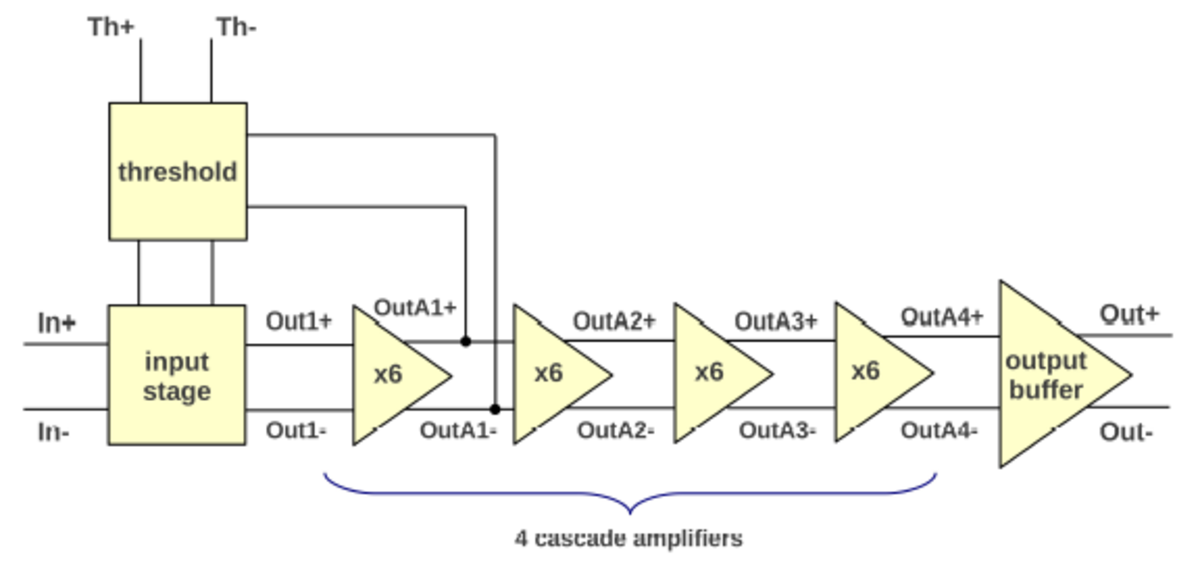
\includegraphics[width=9cm]{Pictures/Chapter_3/NINO_scheme.pdf}\end{center}
\caption[Cascade amplifier of the NINO chip]{Structure of the cascade amplifier of the NINO chip.}
\label{fig:nino_scheme}
\end{figure}

The input stage is a current-to-voltage converter and the subsequent signal amplification is performed with four identical cascade amplifiers that operate as a discriminator as well.
The threshold is set by a voltage difference applied on two symmetrical inputs, as shown in figure \ref{fig:nino_scheme}.
The NINO chip makes use of the time-over-threshold technique: a squared output pulse is produced when the leading edge is above the set threshold, encoding the timing information. The width of this signal, on the other hand, is a function of the charge collected, thus encoding the energy information (see figure \ref{fig:tot}). 
\begin{figure}[htbp]
\begin{center}
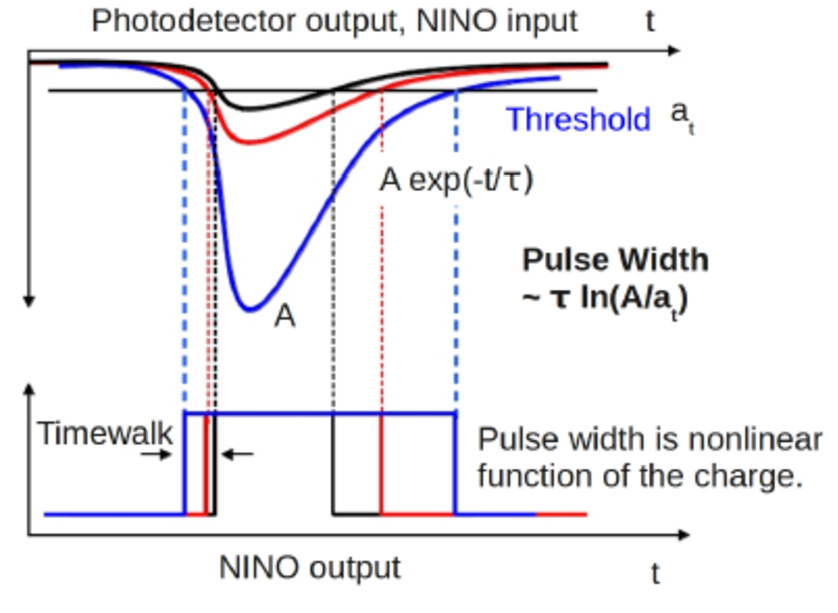
\includegraphics[width=9cm]{../Pictures/Chapter_3/TOT.pdf}
\end{center}
\caption[Time-over-threshold]{Principle of operation of a time-over-treshold discriminator \cite{Gundacker2014}.}
\label{fig:tot}
\end{figure}

}

\chapter{MonteCarlo simulation tools}

\section{Ray tracing}

\section{Geant4}
\subsection{Physics}
\subsection{Implementation}

\section{SLitrani}
\subsection{Physics}
\subsection{Implementation}

\section{A comparison for timing simulation}

\section{Simulation input parameters}
\subsection{Light yield}
The measured light output depends on the absolute yield of the crystal as well as on instrumental and physical factors
\begin{itemize}
\item the temperature dependence of the scintillator output
\item the reflectivity of the wrapping material
\item the condition of the crystal faces
\item the relation between the refractive index of the crystal and the photo detector
\item the quantum efficiency of the photo detector
\item the collection efficiency of the charges produced in the photo detector
\end{itemize}
To measure the light output of sample crystals the number of photo electrons $N_{pe}$ collected can be used.
The number of photo electrons can be calculated by comparison with the position of the photo electric peak with respect to the signal produced by a single photon. The number of photo electron per MeV of the incident $\gamma$ particle can be determined as
\begin{equation}
N_{pe}/MeV=\frac{position\ photo\ peak}{position\ single\ photo\ electron\ peak} \cdot \frac{A_{1}}{A_{2}} \cdot \frac{1}{E_{\gamma}}
\end{equation}
where $E\gamma$ is the energy of the incident $\gamma$ particle and linearity of the detector response is assumed. A pedestal may be subtracted from the position of the peaks. $A_{1}$ and $A_{2}$ are the values of the attenuation of the signal in the case of the photo peak and the single electron peak, i.e.
\begin{equation}
A_{i}=e^{\frac{B_{i}}{20}}
\end{equation}
and $B_{i}$ is the attenuation in dB.

The number of photons emitted per MeV can be determined if the quantum efficiency of the photo detector is known:
\begin{equation}
N_{ph}/MeV=\frac{N_{pe}}{q_{eff}}
\end{equation}
The position of the photo peak and the resolution on the peak are determined with a fit. The fitting function is the sum of a Gaussian and a Fermi distribution:
\begin{equation}
y(x)=\frac{P}{e^{\frac{x-C}{R}}+1}+Ae^{-\frac{(x-\mu)^{2}}{2\sigma ^{2}}}
\end{equation}
where P, C and 1/R correspond to height, position and slope of the Compton edge, A is the height of the photo peak with position $\mu$ and FWHM width $2.35\sigma$. An example of the spectrum fitted with $y(x)$ is shown in figure.


The measurements were performed placing the crystal on top of a \textit{Photonis XP2020Q} photo multiplier tube with the following characteristics:
\begin{itemize}
\item Bi-Alkali photo cathode
\item Refraction index 1.48 (at 420 nm)
\item Peak sensitivity at 420 nm
\end{itemize}
The absorption spectra of the photo cathode is shown in figure.
The quantum efficiency of the PMT was measured experimentally with the following the set up: a light source was sent into a monochromator, the beam was then split in two, and both the PMT to measure and a calibrated photo diode are enlightened. The process was repeated for every wavelength between 250 and 700 nm. The results obtained assessed a quantum efficiency of 0.22 in the UV.

The light output has been measured stimulating scintillation by $\gamma$ rays from a $^{137}$Cs source ($E_{gamma}$ = 662 keV) with an activity of $\sim$ 200 kBq placed a few mm above the crystal. The system crystal-PMT was placed inside a black box, with controlled temperature ($20^{\circ}C$) to avoid drift in the system response.
Further shielding against background light was ensured by an aluminum cap covering the entry window of the PMT.
After the collection of the photo electrons at the anode of the PMT, the signal is attenuated, shaped and stored by the DAQ, with a digitizer \textit{CAEN DT$5720$}.

To correct for long-term variations of the PMT gain and quantum efficiency, the measured light yield was normalized to the light yield of a reference crystal with well known light output.
The reference crystal used is a $2\times 2\times 10$ $mm^{3}$ LuAP crystal encapsulated into Teflon to protect it. In order to normalize the light outputs obtained, the number of photo electrons correspondent to the peak for the reference crystal is required. The number of photo electrons has been evaluated given the single electron response of the crystal. 
The signal produced by a single photo electron and the position of the pedestal were determined by recording the unattenuated PMT signal with the DAQ software: the PMT is covered with a black box and the trigger is lowered to the minimum. The histogram leads to a double peak: one for the electronic noise, one for the single electron. Background noise is due to to charge carriers thermally generated in the electronics and electron released in one of the dynodes by $\gamma$ photons from the source.
The number of photo electrons generated per MeV by the $2\times 2\times 10$ $mm^{3}$ LuAP crystal is $1767$.


\subsection{Optical transmission}
\subsection{Fluorescence spectrum}}
\begin{savequote}[75mm] 
Nulla facilisi. In vel sem. Morbi id urna in diam dignissim feugiat. Proin molestie tortor eu velit. Aliquam erat volutpat. Nullam ultrices, diam tempus vulputate egestas, eros pede varius leo.
\qauthor{Quoteauthor Lastname} 
\end{savequote}

\chapter{Role of crystals in fast timing}

\section{Time profiles}
%vasiliev

\section{The role of Cerenkov photons}
%Serve un calcolo delle soglie per i cristalli usati e i principali parametri

\section{Influence of rise and decay time of TOF-PET}

\section{How to measure: methods}

\subsection{Excitation}
\subsection{Detection}

\section{TCSPC}

\subsection{Statistical and bias problems}

\section{Data analysis techniques}
\subsection{Iterative reconvolution}}
%tutti i cerenkov da mettere

\chapter{A model for scintillation counting}

%role of crystals in fast timing

\section{Signal formation}
%vasiliev

\subsection{Scintillation pulse}
It is customary to describe \cite{Hyman1963} the scintillation pulse as a sum of exponentials. The processes introducted in the previous paragraph, focuse the attention on the alst step of recombination, and the subsequent radiative transitions. 
All the processes that characterize electron hole relaxation and particularly thermalization o the pairs, lead to oscillations with respect to the start of the scintillation pulse determining a non zero rise time.
For all the practcal purposes of this work rise time will be modeled by one or more exponential time components $\tau _{r}$. 
For what concerns recombination, the radiative transitions can be described by one ore more exponential decay times $\tau _{d}$.
In the case of LSO:Ce, for example, the transition takes place between the lowest 5d level, which lies just below the condiction band, and two 4f levels, above the valence band. The parity allowed transition accounts for very fast decay times ($sim$ 40 ns).

We can consider, then, the absorption of a $\gamma$ photon at a time $\theta$. 
For many scintillators, we can describe the probability density function for the emission times as the convolution of two exponential functions representing the energy transfer processes and the radiative decay\cite{Shao2006}:
\begin{equation}
p_{t}(t|\theta) = \int _{-\infty}^{\infty} \exp{\left( -\frac{t'}{\tau _{r}}\right) } \exp{\left(-\frac{t-t'}{\tau _{d}}\right) } \theta (t') \theta (t-t') dt'
\end{equation}
In the case different processes contribute to the scintillation pulse via different energy transfer mechanisms, it may be necessary to consider them\cite{Seifert2012}
\begin{equation}
p _{t}(t|\theta) = \begin{cases} 0, & t < \theta \\ \sum _{i} S_{i} \frac{1}{\tau _{d, i} - \tau _{r, i}} \cdot \left[ \exp{\left( -\frac{t-\theta}{\tau _{d,i}}\right)} - \exp{\left( -\frac{t-\theta}{\tau _{r,i}}\right) } \right], & t > \theta \end{cases}
\end{equation}

\subsection{Cerenkov pulse}


\section{The Cramer-Rao lower bound}
In general, the emission times t of the detected N photons can be considered statistically indipendent and identucally distributed (iid).
Most photo detectors can be modeled as ideal photon counters, able to detect a time stamp for every incoming photon, a set $T_{N} = \{ t_{1}, t_{2}, ..., t_{N}|\theta \}$.

In order to account for the smearing introduced by the resolution of the detector on the photon time stamps, it is necessary to define its response $p_{T}$. In particular  it can be modeled by a Gaussian with a variance equal to the single photon time resolution (SPTR) and a mean equal to the transit time $t_{TT}$. The function is truncated at $t=0$ not to allow negative transit times.
\begin{equation}
p_{T} = \frac{1}{\sqrt {2\pi} \sigma _{SPTR}} \exp{\left[-\frac{-(t-t_{TT})^{2}}{2(\sigma _{SPTR})^{2}}\right]}
\end{equation}
The corresponding pdf for the time stamps is then a convolution of the photon emission rate and the smearing of the detector.
\begin{equation}
p_{t_{n}}(t|\theta) = p_{t}(t|\theta)\ast p_{T}(t)= \int _{-\infty}^{\infty}p_{t}(t-x|\theta) \cdot p_{T}(x)dx = \int _{0}^{t-\theta}p_{t}(t-x|\theta) \cdot p_{T}(x)dx
\end{equation}
And the integral gives
\begin{equation}
p_{t_{n}}(t|\theta) = A \cdot \sum _{i} \frac{S_{i}}{\tau _{d,i} - \tau _{r,i}} \cdot \left[ a_{\tau _{d, i}}(t|\theta) - a_{\tau _{r,i}}(t|\theta)\right]
\end{equation}
where 
\begin{eqnarray}
a _{\tau}(t|\theta) &=& \frac{1}{2} \exp{\left(\frac{\sigma _{SPTR} ^{2} - 2t\tau +2\theta \tau + 2t_{TT}\tau}{2\tau ^{2}}\right)} \\
&& \cdot \left[ erf\left( \frac{t-\theta -t_{TT} - \frac{\sigma ^{2}_{SPTR}}{\tau}}{\sigma _{SPTR}\sqrt{2}} \right) + erf \left( \frac{t_{TT}+\frac{\sigma ^{2} _{SPTR}}{\tau}}{\sigma _{SPTR}\sqrt{2}} \right) \right]
\end{eqnarray}
The Fisher Information $I(\theta)$ is defined as
\begin{equation}
I(\theta) = \int _{-\infty} ^{\infty} \left[ \frac{\partial}{\partial \theta} ln p_{t_{n}}(t|\theta) \right] ^{2} p_{t_{n}}(t|\theta)dt
\end{equation}
Since the samples are iid, the information is additive, so that
\begin{equation}
I(\theta) = N \cdot \int _{-\infty} ^{\infty} \left[ \frac{\partial}{\partial \theta} p_{t_{n}}(t|\theta) \right] ^{2} \frac{1}{p_{t_{n}}(t|\theta)}dt
\end{equation}
The Cramer Rao theorem states that the variance of any unbiased estimator $\hat{\theta}$ of $\theta$ is bounded by the reciprocal of the Fisher information:
\begin{equation}
var(\hat{\theta})\geq \frac{1}{I(\theta)}
\end{equation}
In a PET-like experiment the interest lies in the estimate of the photon time of interaction $\theta$.
Statistically speaking the Cramer Rao theorem gives the intrinsic time resolution limit for any given scintillator with the given parameters.

\section{The order statistics}
If it is assumed a specific order in the set of recorder timestamps, it is evident that they are neither independent nor identically distributed. By sorting the elements in $T_{N}$ we can create an ordered set $T_{\bar{N}} = \{ t_{\bar{1}} \leq t_{\bar{2}} \leq ... \leq t_{\bar{N}} \}$. The pdf for the nth-order statistics is given by\cite{Seifert2012}
\begin{equation}
f_{n}|N (t\theta) = \binom{N}{n} \cdot n \cdot P_{t_{n}}^{n-1}(t|\theta) \cdot \left[ 1-P_{t{n}}(t|\theta) \right] ^{N-n}\cdot p_{t_{n}} (t|\theta)
\end{equation}
In this case the set is not iid; thus considering an estimator using a unique timestamps, as the case of analog SiPMs, the Fisher information is
\begin{equation}
I_{n}(\theta) = \int _{-\infty} ^{\infty} \left[ \frac{\partial}{\partial \theta} ln f_{n}(t|\theta) \right] ^{2} f_{n}(t|\theta)dt
\end{equation}
   
\section{Intrinsic time resolution}

% parametri che variano, lower bound (compresi i cerenkov, anzi di' subito che contano poco e niente)

\section{Effects on signal extraction}

% qui vai a vedere il singolo fotone in basso, dato un sipm
}
\chapter{Na-22 measurement}

In a PET system the excitation energy of the incident $\gamma$ is 511 KeV. As stated previously, at this energy a series of different processes intervene and contribute to the time resolution measured.
Three elements should be considered, when comparing time profiles to the one measured with VUV radiation:
\begin{itemize}
\item production of Cerenkov photons
\item volume excitation (and so transit time spread in the bulk)
\item de excitation down to the thermalization region
\end{itemize}
The relative strengths of these phenomena have already been compared in chapter 6, and the possibility of measuring at high energy allows to phisically quantify these effects.
In particular a TCSPC system based on a $^{22}$Na source has been implemented, using a tagging crystal and a SiPM as a start signal and a MCP-PMT as a stop signal. 

\section{Phenomenology}

The physics of $\gamma$ photon interaction have been already introduced in chapter 2.
In order to build a time correlated single photon counting experiment two time signals are necessary, a start signal and a stop signal.
A simple way to obtain this is to use a $\beta ^{+}$ active isotope, such as $^{22}$Na. This isotope emits a positron according to the decay reaction $^{22}Na \rightarrow ^{22}Ne + \beta ^{+} + \nu _{e} + \gamma$. The positron yield is relatively high, $90.4\%$, and competitive processes are electron capture (EC) and direct transition to the Ne ground state. 
In the positron emission case the Ne ground state is reached after 3.7 ps by emission of a $\gamma$ quantum of 1.274 MeV. The half life of the isotope is 2.6 years.
\begin{figure}[htbp]
\begin{center}
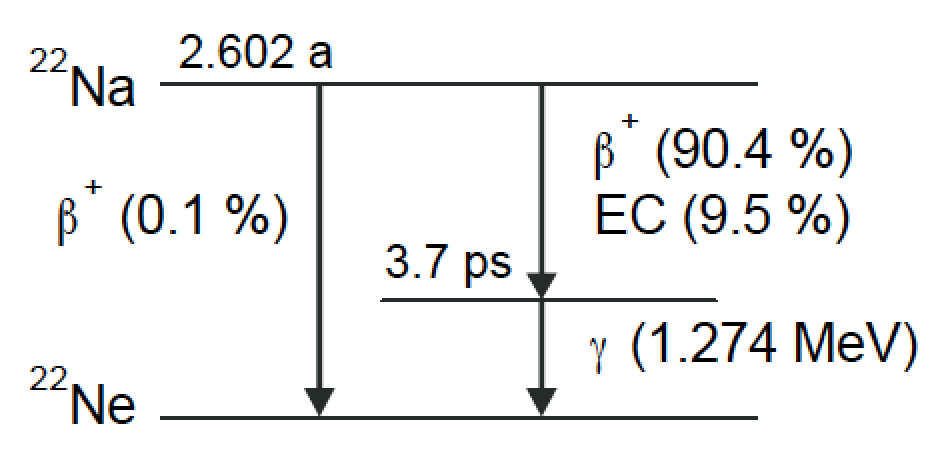
\includegraphics[width=8cm]{../Pictures/Chapter_8/Na-22}
\end{center}
\caption[Na$^{22}$ decay scheme]{Decay scheme of Na$^{22}$}
\label{fig:Na_22}
\end{figure}
It is worth to note that, as outlined in chapter 2 the Cerenkov threshold for heavy scintillators is below the energy of the annihilation $\gamma$ produced by the isotope.

\section{Experimental setup}

\begin{figure}[htbp]
\begin{center}
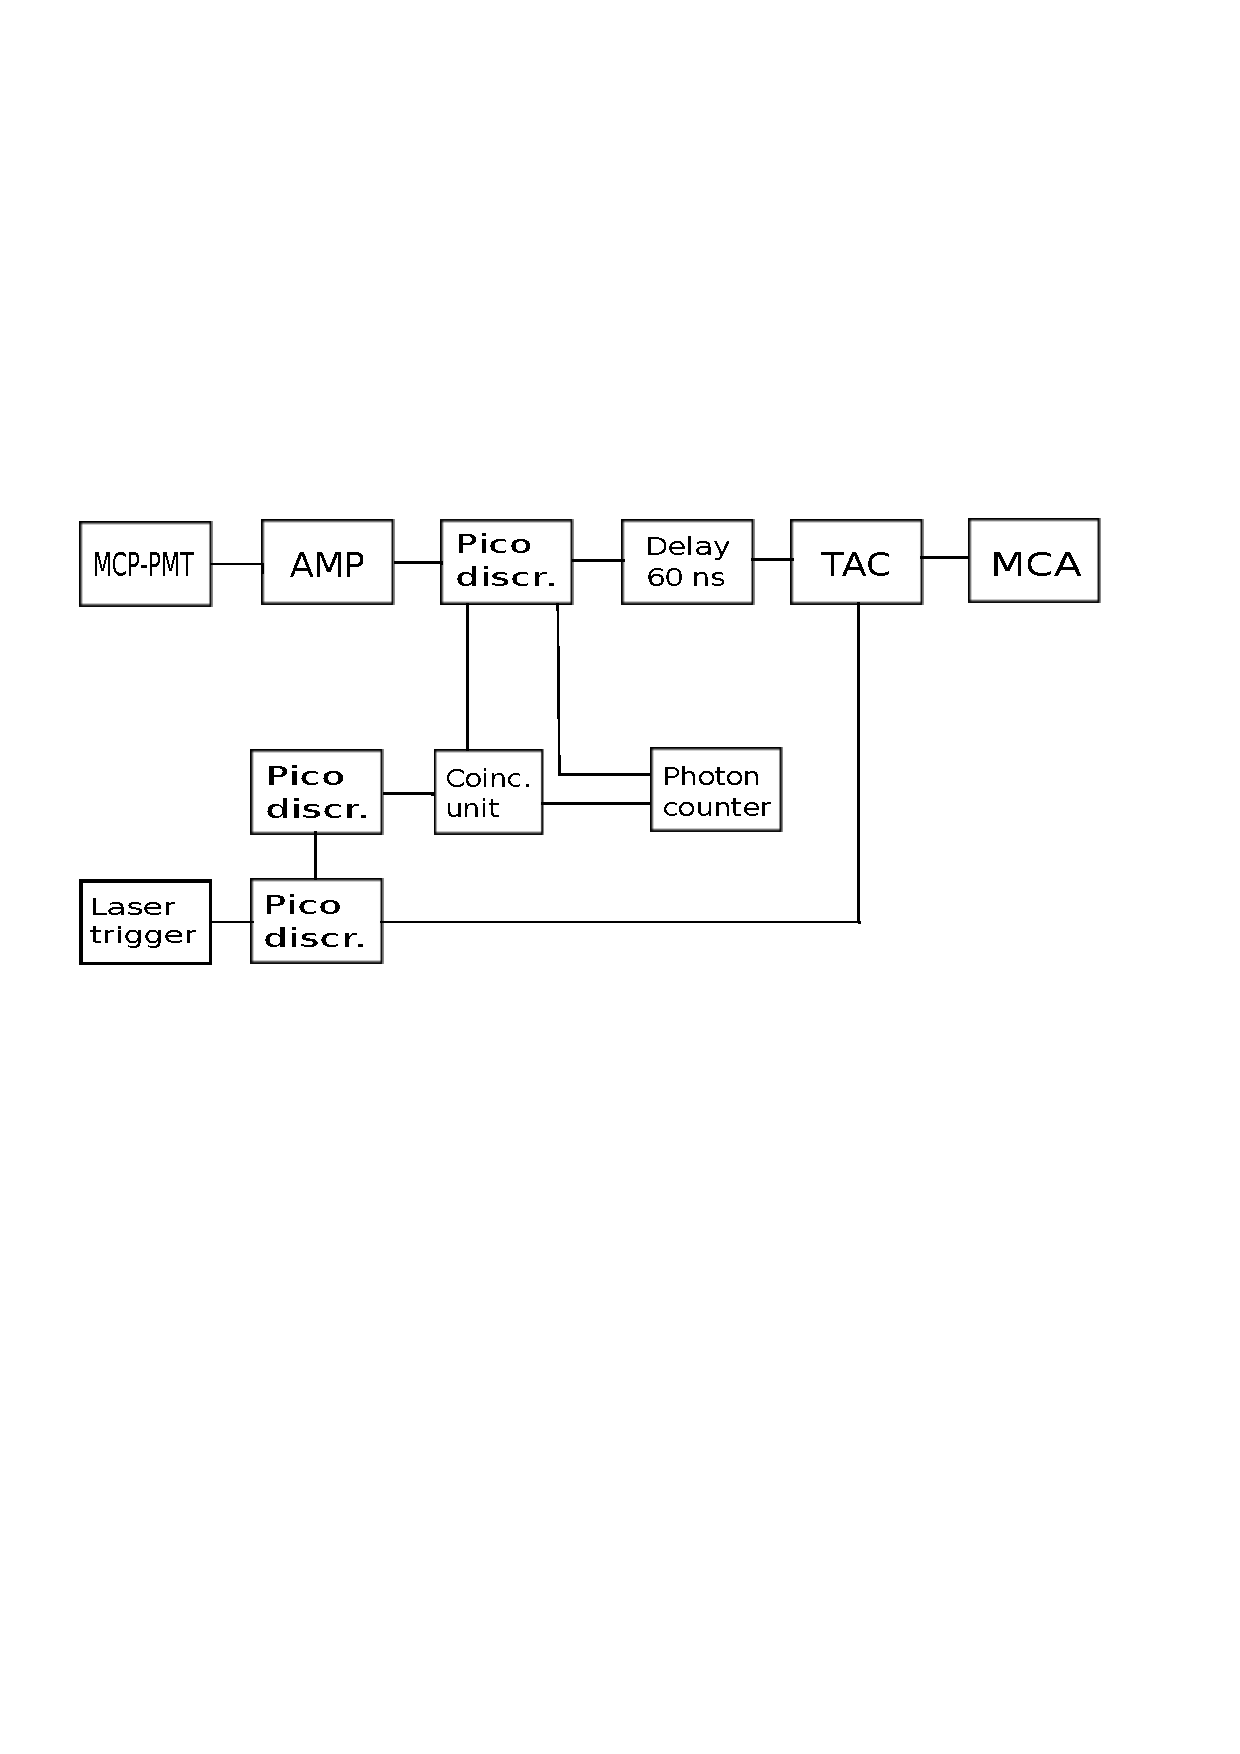
\includegraphics[width=8cm]{../Pictures/Chapter_8/electronics.pdf}
%qui una bella foto?
%\includegraphics[width=8cm]{../Pictures/Chapter_8/electronics.png}
\end{center}
\caption[Setup for $\gamma$ measurement]{The setup and DAQ for the $\gamma$ measurement is shown.}
\label{fig:setup}
\end{figure}
The scheme of the setup is shown in figure \ref{fig:setup}.
The tagging crystal used in this configuration is a 2x2x5 mm$^{3}$ LSO:Ce,Ca pixel, readout by a SiPM board amplified by a NINO chip. 
% glue? cerca misure del mppc!
The SiPM mounted on the board is a 3x3 mm $^{2}$ Hamamatsu MPPC S10931-050P with 50 $\mu$m cell size.
Its signal is then fed in to the NINO chip described in chapter 3. The NINO technology, thanks to the time-over-threshold technique, collects time and energy information at the same time, thus allowing for a complete cut analysis.
The SiPM was biased through the board at 72.5 V, and the NINO at the nominal working voltage of 2.5 V. Moreover a potentiometer installed in the board allows to set up the lower and higher threshold for the NINO chip, as will be discussed in the following paragraph.
The signal is directly coupled to a high-bandwidth oscilloscope, able to digitize the pulses, a LeCroy DDA 735Zi (10 GS/s).
A sample of the NINO signal is shown in figure \ref{fig:NINO_sign}.
\begin{figure}[htbp]
\begin{center}
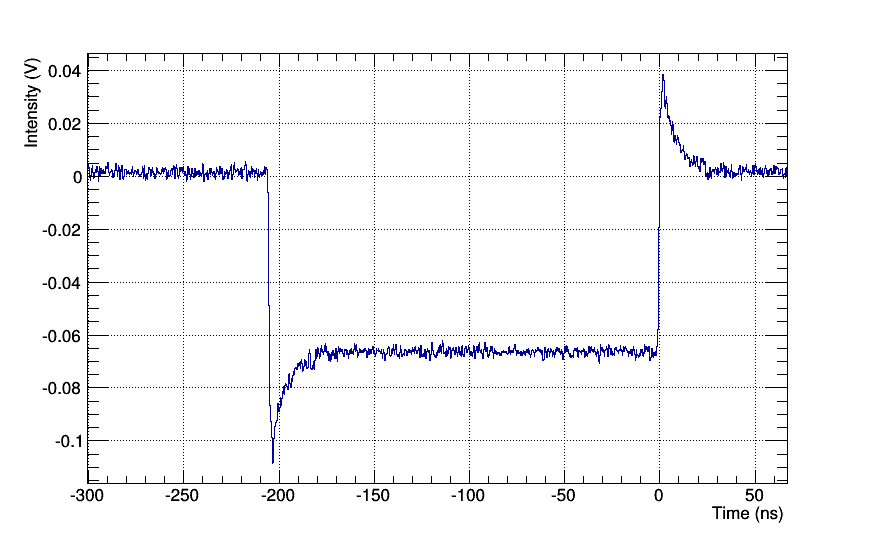
\includegraphics[width=8cm]{../Pictures/Chapter_8/NINO_signal.png}
\end{center}
\caption[NINO signal sample]{Example of NINO output from SiPM signal.}
\label{fig:NINO_sign}
\end{figure}
The stop signal is directly routed in to the oscilloscope without amplification. The stop detector is a Hamamatsu R3809U-50 MCP-PMT.
The signal of the MCP is very fast, as can be seen in figure \ref{fig:MCP_sign}, since it is almost completely contained in 1 ns. This allows for a multi photon detection setup.
Indeed the two signal lines from the oscilloscope were saved for offline analysis, acting as a completely digitalization of the signal.
\begin{figure}[htbp]
\begin{center}
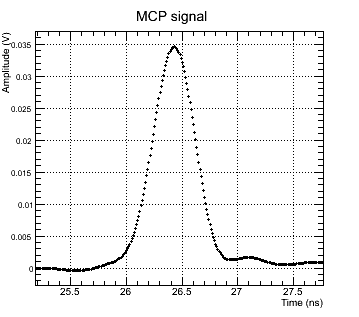
\includegraphics[width=8cm]{../Pictures/Chapter_8/MCP_signal.png}
\end{center}
\caption[MCP signal sample]{Example of Hamamatsu MCP-PMT output.}
\label{fig:MCP_sign}
\end{figure}
The components of the apparatus were placed in a cooled light-tight box, and the temperature held at 20 $^{\circ}$C with a degree tolerance.
Cooling is necessary to mantain the performance of SiPM. Indeed the number of thermal electrons that give rise to dark counts in the detector is strongly dependant on the temperature.
In the setup presented, as already pointed out, the accumulation times can be quite slow. It is necessary to keep the number of detected photon low, so that no significant bias is introduced in the measurement. The number of starts is thus much bigger than the number of stop at the acquisition. In order to gather data for a reasonable accumulation time, it is essential to reduce to the minimum the time the acquisition system (i.e. the oscilloscope) is busy.
The MCP benefits from temperature stability as well, and for the same reasons, but the noise level is negligible if compared to the SiPM.
Moreover the threshold set for the SiPM plays an important role on the DCR level of the device: in this case the DCR at 200 mV threshold is 0.88 Mcps (for complete discussion see \cite{Gundacker2014}). 

% cita gundi e piazza il valore
%spiegare e mostrare il setup della board cioe come funziona e perche quelle soglie

\section{Preliminaries}

In order to extract the parameters leading to the determination of rise time values and to critically analyze the impulse response funciton measured, the properties of the start and stop detectors were separately measured. 
In a second phase, the impulse response function was measured, without the sample, as it is a crucial part for the iterative reconvolution routine.
Finally the bias fraction for an optimal count rate for the sample measured was assessed.

\subsection{Characteristics of the start signal}

As already outlined, the start signal originates in a tagging crystal.
The crystal is a 2x2x5 mm$^{3}$ LSO:Ce, Ca pixel, glued to the SiPM. Between 4500 and 5000 photons are collected at the photodetector, already corrected for the quantum efficiency. 
%e'vero?
The working point for the NINO chip, biased at 2.5 Volts, was set via a potentiometer on the board, at 200 mV.
% no le threshold non sono capite!
The signal is selected at the photopeak, so that the contribution from time walk is limited.
In order to estimate the contribution of the start signal to the total IRF the board was measured in CTR along with a reference board.
The setup for CTR measurement is a simple start-stop configuration with two similar boards and a $^{22}$Na source.
The reference board was measured separately and details will not be given here, for a complete discussion see \cite{Gundacker2014}. The CTR on the reference arm is $\sim$ 105 ps FWHM, measured after selection at the photopeak on both arms, as shown in figure \ref{fig:start}.
In the same figure the $^{22}$Na spectrum in LSO is shown, with the single photon signal at the beginning of the range. Non linearity due to the time over threshold technique are present, although not taken into account separately. Since the best time resolution is delivered in the photopeak region, the influence of non linearity in the energy spectrum is negligible. 
\begin{figure}[htbp]
\begin{center}
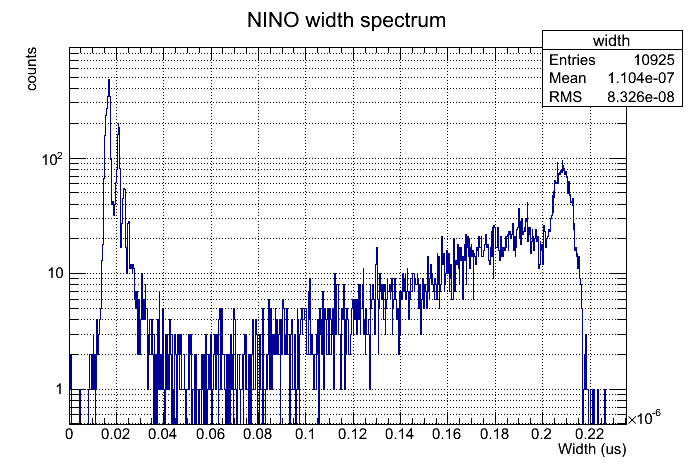
\includegraphics[width=7cm]{../Pictures/Chapter_8/spectrum_NINO.png}
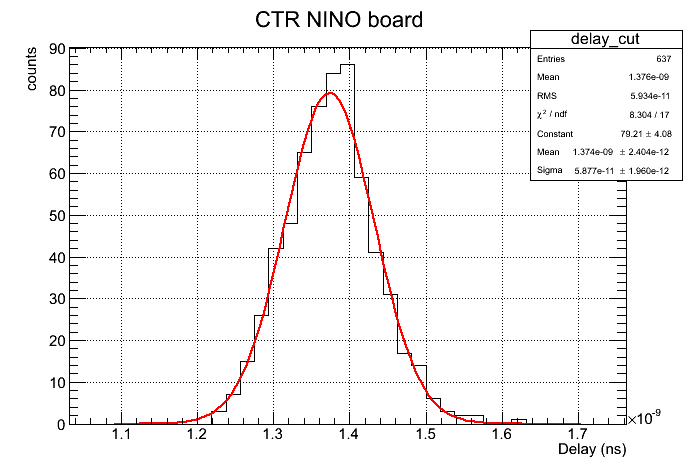
\includegraphics[width=7cm]{../Pictures/Chapter_8/CTR.png}
\end{center}
\caption[Start characteristics]{Example of start spectrum (left) and measured CTR at the photopeak (right).}
\label{fig:start}
\end{figure}

The electronics contribution depends on the data aquistion electronics and its noise level. This contribution can be estimated as
\begin{equation}
\sigma _{noise} = \frac{RMS _{noise}}{dV/dt}
\end{equation}
where the RMS of the noise is determined from the pedestal of the signal and $dV/dt$ is the slew rate. In this case it can be estimated at 37 ps (for a complete discussion see \cite{Gundacker2014}). 

\subsection{Characteristics of the stop signal}
The stop signal is a is a Hamamatsu R3809U-50 MCP-PMT. In order to estimate the contribution of the stop signal to the total IRF the MCP time response was measured with the aid of a high resolution laser.
The setup is composed by a Picosecond Diode Laser-Pilas head and a series of optical filters to reduce the light intensity hitting the photodetector down to less than one photon per excitation. The two signal are than routed to a LeCroy Oscilloscope LeCroy DDA 735Zi (10 GS/s) and data analysis is performed offline.
In order to measure the MCP SPTR a high resolution laser is needed, matching the wavelength of emission of the scintillator measured in TCSPC, if possible. The Pilas laser delivers a 28.9 ps pulse (FWHM) at a frequency of 100 kHz and a wavelength of 419 nm. The rising edge of the laser trigger is shown in figure \ref{fig:trigger}.
\begin{figure}[htbp]
\begin{center}
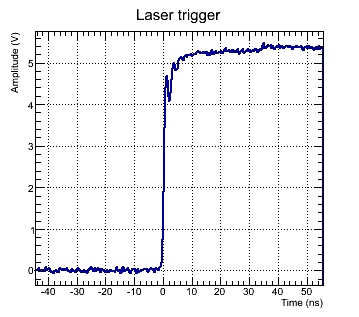
\includegraphics[width=8cm]{../Pictures/Chapter_8/laser_trigger.png}
\end{center}
\caption[Laser trigger]{Rising edge of the laser trigger.}
\label{fig:trigger}
\end{figure}
To extract the time difference between the laser trigger and the MCP signal, an offline analysis was performed. The digitized pulses were saved and analyzed with the software package ROOT. A threshold for trigger was set at 5 mV on the MCP and the time difference was calculated in the interpolated signal. Therefore the sampling of the signal goes from 10 GS/s to 100 GS/s. 
\begin{figure}[htbp]
\begin{center}
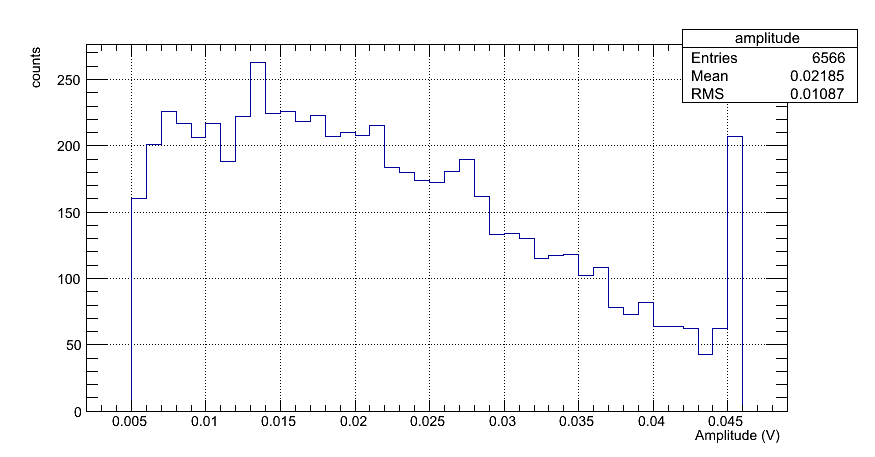
\includegraphics[width=7cm]{../Pictures/Chapter_8/amp_MCP.png}
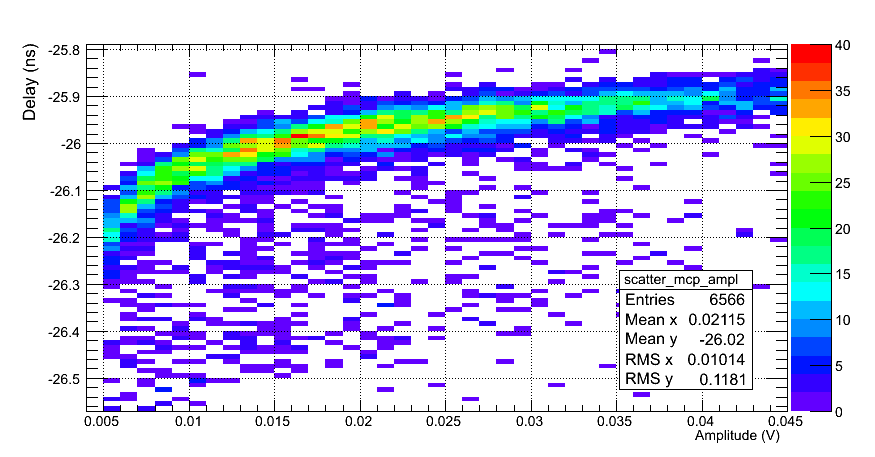
\includegraphics[width=7cm]{../Pictures/Chapter_8/time_walk_mcp.png}
\end{center}
\caption[Time walk of the MCP-PMT]{Amplitude spectrum for the MCP-PMT (left) and scatter plot amplitude - delay (right).}
\label{fig:mcp_laser}
\end{figure}
As shown in figure \ref{fig:mcp_laser}, the amplitude of the MCP varies considerably on the range considered, that is between 5 mV and 50 mV, where most of the signals lie. A saturation effect due to the limited amplitude window of the oscilloscope is also present, but cut in data analysis. This variation makes the stop detector prone to important time walk. 
The possibility of storing separately the digitized pulses allow for a complete selection and correction of these events. The scatter plot in figure \ref{fig:mcp_laser_walk} is corrected through a simple time walk correction.
If we define the real time stamp brought by the signal as t$_{real}$, the threshold crossing time t$_{measured}$ and the jitter given by the time walk we can write
\begin{equation}
t_{ideal} = t_{measured} - t_{walk}
\end{equation}
and we can extract the walk correction as
\begin{equation}
t_{walk} = A + B\cdot E^{C}
\end{equation}
where E is a measure of the charge collected. In this case it will be the amplitude of the MCP-PMT signal.
\begin{figure}[htbp]
\begin{center}
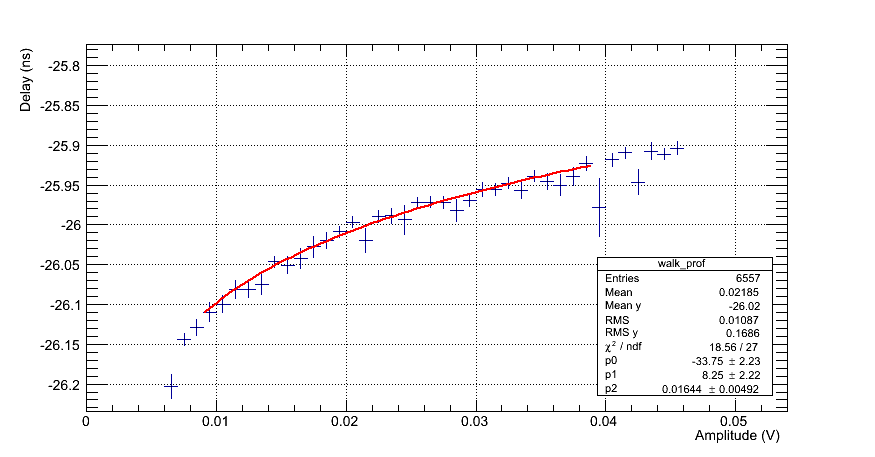
\includegraphics[width=7cm]{../Pictures/Chapter_8/time_walk_corr.png}
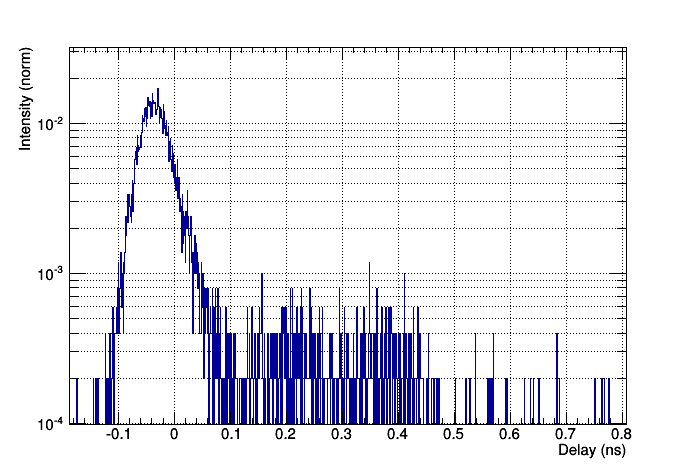
\includegraphics[width=7cm]{../Pictures/Chapter_8/laser.png}
\end{center}
\caption[MCP corrected response (laser trigger)]{Time walk correction on the spectrum profile, MCP-PMT against laser trigger (right) and resulting corrected response (right).}
\label{fig:mcp_laser_walk}
\end{figure}
At this point the spread on the time difference spectrum shown in figure \ref{fig:mcp_laser_walk} is given by four phenomena:
\begin{itemize}
\item width of the laser signal
\item jitter on the laser trigger
\item SPTR of the detector
\item electronics noise
\end{itemize}
It is natural to consider this processes uncorrelated so to concur to the smearing of the time distribution as
\begin{equation}
\sigma _{TOT}^{2} = \sigma _{SPTR}^{2} + \sigma _{laser}^{2} + \sigma _{trigger}^{2} + \sigma _{noise}^{2} 
\end{equation}
The laser width was taken from the datasheet, and amounts to 30 ps FWHM. The laser trigger can be substantially neglected as it amounts for $\sim$ 4 ps FWHM. Given the slew rate of the signal the $\sigma _{noise}$ amounts to $\sim$ 10 ps.

The spectrum measured can be grossly modeled as a Gaussian with a tail towards high delays. 
We notice from figure \ref{fig:mcp_laser} that ion feedback modifies the signal at higher times but it is almost two order of magnitude lower than the peak, as it is expected from a Chevron configuration. Considering the Gaussian peak we find $\sigma _{TOT} =$ 25 ps, so that we can infer    $\sigma _{SPTR} = $ 18 ps, given that $\sigma _{noise}^{2}$ amounts to 10 ps and $\sigma _{laser}^{2}$ to 13 ps.

\subsection{IRF measurements}
The last step is the measurement of the impulse response function (IRF), that is global variance on the estimate of the time stamps given by the combined effect of the start and stop uncertainties. This time spectrum needs to be deconvolved from the time spectrum of the sample measured in order to extract the parameters of the fluorescence.
In order to estimate the impulse response function, the set up presented in the previuos section was used without the scintillation sample. The start signal retains the same characteristics, but the stop signal is given by a direct interaction in the MCP-PMT. This allows to disentagle the measured curve from the effect of the crystal, time constants and travel spread of the photons.
\begin{figure}[htbp]
\begin{center}
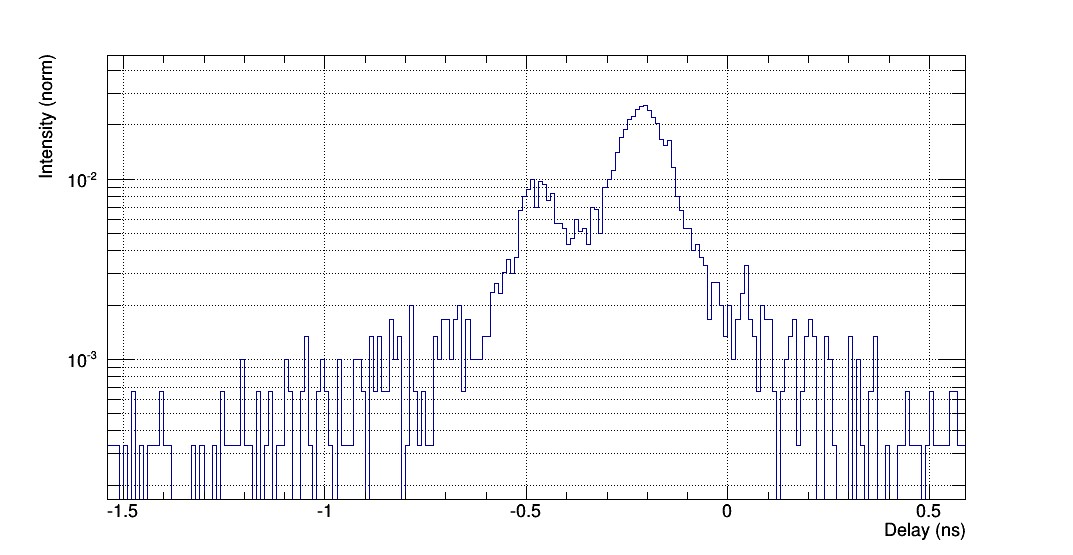
\includegraphics[width=8cm]{../Pictures/Chapter_8/response_cer_10}
\end{center}
\caption[Corrected IRF]{Measured response of the stop signal (MCP) against start signal (SiPM).}
\label{fig:ceren_10}
\end{figure}

The time walk corrected time spectrum is shown in figure \ref{fig:ceren_10}. Two separable components are present, separated by $\sim$ 300 ps. %?
In this configuration, The processes that concur to the time spectrum are:
\begin{itemize}
\item Cerenkov photons produced by $\gamma$ photons impinging in the entry window of the MCP-PMT
\item direct interaction of the $\gamma$ photons in the MCP stack
\end{itemize}
The delay of the two processes is contained in a time window of $\sim$ 300 ps.
Given the large variation in the output signal of the MCP it is not possible to select event by event with a pulse shape rejection method.
Using a simple Geant4 simulation it is possible to show that Cerenkov photons produced in the window need to interact in the photocathode and then allow time for the produced photo electron to travel in the electric field to the MCP stack. On the left side of figure \ref{fig:drift} the times of Cerenkov production in the entry window and the time of a $\gamma$ photon interaction in a MCP stack is shown.
\begin{figure}[htbp]
\begin{center}
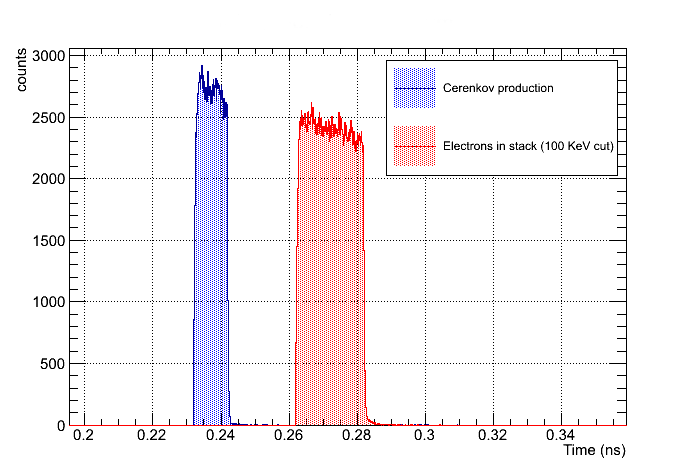
\includegraphics[width=7cm]{../Pictures/Chapter_8/interaction_time_spectrum.png}
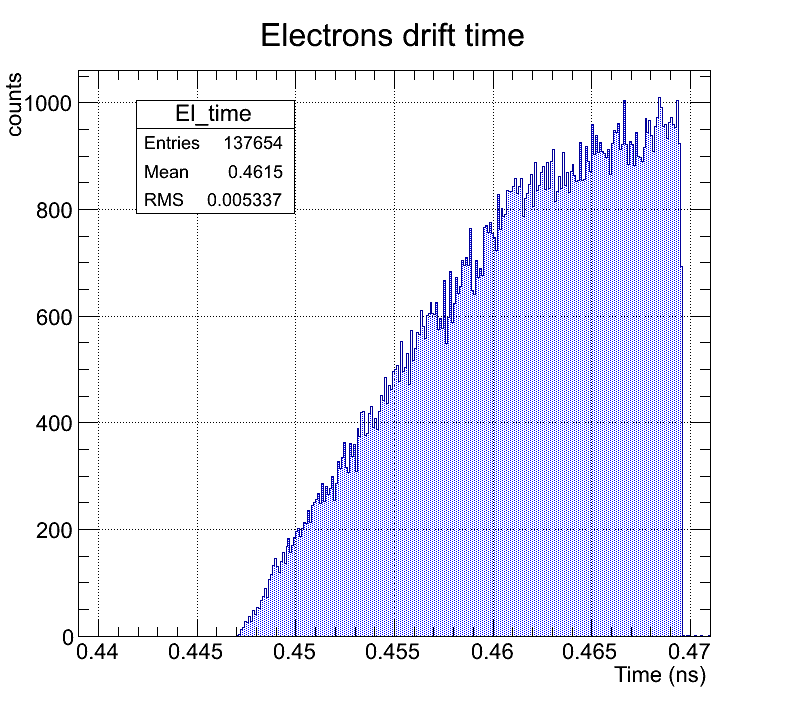
\includegraphics[width=7cm]{../Pictures/Chapter_8/electron_drift.png}
\end{center}
\caption[Stack and Cerenkov simulation]{Time of interaction simulate for MCP stack and entry window Cerenkov photons (left) and drift time of electrons after the photocathode (right). }
\label{fig:drift}
\end{figure}
It is then necessary to add the drifting time of the electrons between the photocathode and the first MCP stack, based on the geometry of the detector. The drifting electric field by design is given by the voltage divider of the detector, and amounts to 310 kV/m.
As shown on the right side of figure \ref{fig:drift} the drifting time of the electrons matches the time difference in the two components present in the measured IRF, and small deviations can be ascribed to partial knowledge of the detector materials and geometry of the electric field in the drifting region.

This phenomenon can be experimentally shown by selectively suppress one of the two processes. The setup was then slightly changed by tilting the MCP-PMT with respect to the start-source system.
\begin{figure}[htbp]
\begin{center}
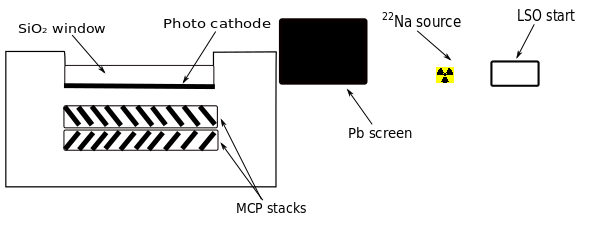
\includegraphics[width=7cm]{../Pictures/Chapter_8/screen_irf_2.png}
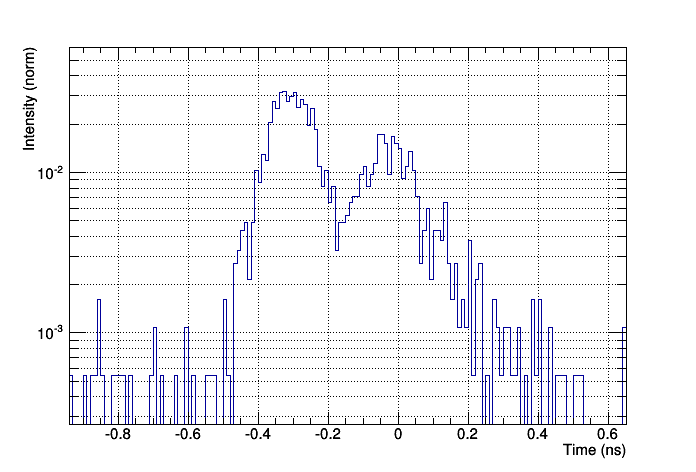
\includegraphics[width=7cm]{../Pictures/Chapter_8/turn_1.png}
\end{center}
\caption[Setup for $\gamma$ interaction in stack]{Setup for $\gamma$ interaction in stack (left) and spectrum recorded (right)}
\label{fig:twist2}
\end{figure}
\begin{figure}[htbp]
\begin{center}
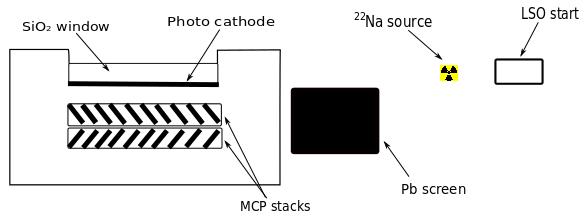
\includegraphics[width=7cm]{../Pictures/Chapter_8/screen_irf.png}
\includegraphics[width=7cm]{../Pictures/Chapter_8/turn_2.png}
\end{center}
\caption[Setup for Cerenkov production in the window]{Setup for Cerenkvo production in window (left) and spectrum recorded (right)}
\label{fig:twist1}
\end{figure}
Then a lead screen was placed in between and two set of measurements was performed, as shown in figure \ref{fig:twist1}:
\begin{itemize}
\item a first one with the screen covering the direct line of interaction between the source and the position of the MCP stack deduced from the design of the detector
\item a second one with the screen covering the section of the entry window
\end{itemize}
It was then possible to suppress, respectively, the direct $\gamma$ interaction in the stack and the Cerenkov production in the window. The relative intensity of the two peaks is reversed, as shown in figure \ref{fig:twist2}. 
The final time resolution can be inferred from the 
last figure, since the IRF to be deconvolved is composed only by the part of the spectrum related to photo electrons. As will be explained below, the direct interaction of $\gamma$ photons in the stack brings additional spurious background to the spectrum, but it is not related to the scintillation pulse. Nevertheless the two peaks show similar width, and this is due to the fact that the resolution is dominated by the start signal, which is far worse and the slight difference given by the electron drift is negligible.
As a consequence, we cut on the Cerenkov part of the IRF spectrum, and extract the width as a $\sigma _{IRF}$ = 73 ps. This is in substantial agreement with the discussion of the previous section since $\sigma _{IRF}^{2} = \sigma _{stop}^{2} + \sigma _{start}^{2} + \sigma _{noise}^{2}$, where $\sigma _{start}$ = 62 ps, $\sigma _{noise}$ = 37 ps and $\sigma _{stop}$ = 18 ps.

\subsection{Control of the bias fraction}
The main advantage of using the available oscilloscope as a digitizer of the pulses for offline analysis is the possibility of extracting multi time stamps. This allows for a multi-hit TDC approach. 
Thanks to the fact that signals from MCP-PMT are very fast, i.e. completely contained in 1 ns, the dead time is very low and so it is the biased fraction of events. 
Starting from the considerations previously stated in chapter 6, it is possible to control this fraction by counting the number of pulses per event.
Usually the biased fraction is qualitatively controlled by calculating the geometric factor of the setup and by keeping the number of counts well below one per start signal. This was also the approach used in the case of VUV measurement, where  no multi hit TDC was available.
In the case of the $\gamma$ setup, also given the low number of counts and the difficulties in collecting a high statistics, it is necessary to keep the rate as high as possible, while still being sure not to introduce significative bias in the measurement.
In this setup it is possible to control in real time the number of pulses per event that should follow a Poisson distribution, as shown in figure \ref{fig:} for a LSO:Ce, Ca crystal. The extraction of the average allows to completely control the bias fraction, and this was done for all the samples measured.
\begin{center}
%\includegraphics[width=7cm]{../Pictures/Chapter_8/.png}
\includegraphics[width=7cm]{../Pictures/Chapter_8/multi_pois.png}
\end{center}
\caption[Multi hits in $\gamma$ setup]{Example of multi hit event (left) and distribution of pulses over the events (right).}
\label{fig:twist1}
\end{figure}
\subsection{Background}
In the measurement campaign conducted two separate background processes intervene:
\begin{itemize}
\item random coincidences
\item direct interaction of a $\gamma$ in the detector
\end{itemize}
For what concerns random coincidencies they should be kept at a low level, in order not to worsen the uncertainty on the parameter extraction at the fit level. Indeed the important parameter is the signal to noise ratio and this aspect depends strongly on the light yield of the crystal measured, and on the geometry of the system. Nevertheless this kind of event is taken into account in the fit procedure, and in principle the only disadvantage is the necessity for higher statistics to be collected.

The direct interaction of a $\gamma$ in the detector, on the other hand, could severely bias the measurement, in the time window where the rising edge of the crystal lies. 
The active area of the MCP is quite large, given the size of the entry window, with a diameter of 11 mm. This makes direct interaction in the detector quite likely.
This is easily taken in to account in the case of 511 KeV $\gamma$, since they are emitted back to back. In this case it is sufficient to tilt the stop detector with respect to the sample to measure, with an angle of 90 $^{\circ}$C.

As previously explained, in addition to the 511 KeV $\gamma$ photons produced by the annihilation of the positron, the $^{22}$Na de-excite to the $^{22}$ Ne ground level by emitting a 1.274 MeV $\gamma$. 
The de-excitation $\gamma$ is emitted isotropically and can interact in the detector after a gate is open on the start arm, unrelated to any scintillation event in the sample.
As shown in \ref{fig:twist2} this events happen exactly on the rise time of the signal, since the delay introduced by the geometry is negligible.
It is not possible to select on a pulse shape basis since the MCP amplitude largely varies, and there is no separable difference between signals coming from a 1.274 MeV event and a photo electron event.

Thus in order to restrict the influence of this events, which become less and less problematic as light yield of the sample measured increase, two approaches are possible:
\begin{itemize}
\item screen the detector from the source
\item optically delay the scintillation light in order to easily cut spurious events from direct interaction.
\end{itemize}
The first solution was chosen for time constraints, but the optical delay will be implemented in the future. In particular 5 cm of lead blocks were positioned in between, that allow to stop 95$\%$ of the incoming $\gamma$ photons (density and stopping power taken from \cite{nist2005}). This is the case shown in figure \ref{fig:twist3} for CeF$_{3}$.

\begin{figure}
\begin{center}
%\includegraphics[width=7cm]{../Pictures/Chapter_8/.png}
\includegraphics[width=7cm]{../Pictures/Chapter_8/setup_direct.png}
\end{center}
\caption[Background biased measurement]{Highly biased time profile of CeF$_{3}$ sample (left) and relative setup (right).}
\label{fig:twist2}
\end{figure}

\begin{figure}
\begin{center}
%\includegraphics[width=7cm]{../Pictures/Chapter_8/.png}
\includegraphics[width=7cm]{../Pictures/Chapter_8/setup_twist.png}
\end{center}
\caption[Background suppressed measurement]{Background suppressed time profile of CeF$_{3}$ sample (left) and relative setup (right).}
\label{fig:twist3}
\end{figure}

\section{Data analysis}
Due to time constraints not all the samples measured in VUV could be measured with the $\gamma$ setup, though the proof of concept was delivered for future completion of the study.
The samples measured in the $\gamma$ setup were
\begin{itemize}
\item LYSO 2737
\item LGSO
\item CTI 2408
\item CeF3
\item LSO Ca Ce
\item LuAG %?
\end{itemize}
The data extracted were analyzed offline for cuts and time walk correction. 
The rise time parameter was extracted with the iterative reconvolution algorithm presented in chapter 6, and the error was evaluated as confidence interval on the $\Delta$Likelihood.

\subsection{Cuts and background estimation}
The IRF measurement was performed at the beginning of the campaign and repeated at regular intervals to correct for eventual drifts, but no significant drift was observed.
On the data collected for offline analysis the first cut performed is the photopeak selection on the start signal, that for the NINO signal happens between 200 and 220 ns, at the 511 KeV peak of the $^{22}$Na.

For the MCP data two set of manipulations were perfomed: on the amplitude of the MCP to avoid saturation effect and for time walk correction. 
The MCP signal was cut between 10 and 40 mV, which is the interval that contains the 70$\%$ of the pulses collected. At this point the signal was corrected for time walk.

As previously explained, the background can play an important role in the measurement, especialli in the case of crystals with low or very low light yield, which is the case of CeF$_{3}$ for example. 
In order to control this a lead screen was positioned between the source and the MCP to suppress the count rate from direct interaction in the stack. Additionally a quick background measurement was performed, to ensure that the background count rate could be neglected.

\subsection{Fit procedure}

\subsection{Results}
\subsection{Summary}}
%==============================================================================

%-----------------------------------------------------------------------------%
% APPENDICES -- OPTIONAL. These are just chapters enumerated by Appendix A,
%                Appendix B, Appendix C...
%-----------------------------------------------------------------------------%
\appendix
\chapter{Populo Ornatus}

Ut quando convenire scripserit mei, ut accusam noluisse eam. At scripta democritum quo, reque everti an qui, posidonium efficiendi ut mel. Pro an reque habemus, augue nemore conceptam in vim. Eu cibo ancillae takimata usu.

No vis albucius rationibus, eum doming ceteros constituto id. Ad suas zzril laudem cum. Natum mollis singulis vel te, ea elit imperdiet duo, odio inermis et eos. Nam ad vocibus tractatos, sit no vidisse diceret omnesque, mollis omnesque ea mea.

Ut est ridens principes scribentur, menandri interesset adversarium ius ut. Ut duo elit dissentias, at sea eleifend scripserit, eam nibh rebum definitiones an. Cum te quaeque epicuri mentitum, his elitr essent et, in sea habeo aliquid convenire. Quo euismod sadipscing definitionem an, ut duo iusto aliquando, graece appetere ne nec.

Consul imperdiet dignissim vis et, mei liber vidisse principes et, eu nam docendi voluptua democritum. Qui no dicat tamquam sanctus, saepe tincidunt no mel. Pro ignota albucius consetetur in, sint qualisque assueverit eam ut, vis graeco denique signiferumque ne. Sale appellantur contentiones eu his, pro magna ornatus ut, ad vidit omnesque euripidis pri. Sea congue moderatius in, his dicit suscipit no, mei ei incorrupte assueverit. Nusquam nominavi et quo, idque delenit vim an, posse quaeque an mea.

Suas elitr lucilius sit an, aeterno persius vel eu. Mel at essent aperiam repudiare. Tale consul eum ne, eam no meis delenit iudicabit, an sint mutat pri. Nec no clita propriae pericula, duo explicari gubergren ei. Ne sit autem nominavi, te falli deserunt per. Quo tractatos suscipiantur ex, electram dignissim usu no, cu congue iriure vivendo vim.

At vero graeci fuisset his, quo similique persequeris ad. Ex est graece mandamus, antiopam voluptatum his ea. Assum appellantur mel an, ei mea veri commune efficiendi. Pri blandit urbanitas no. Nam ex enim reque, ut nec iusto regione ullamcorper, facer harum pertinacia mei ei. Erant veniam imperdiet an eam, veniam mucius equidem ius eu, at scripta labitur est.

Et quo soluta graecis accommodare. Tamquam mentitum menandri vim ut. Ut nec melius senserit, ut mei sale aeque. Prompta delectus mea te, fierent adipisci ad per, mei odio pertinax senserit et. Per ut persius singulis. Id qui malorum iracundia, semper conceptam cu sed.

Vis nominavi urbanitas intellegat an, ut numquam deseruisse sea. Et quo dico aeque adipiscing, ius ea commodo epicurei, eum cu nulla imperdiet efficiantur. Ea cum simul scripserit. Ius reque decore voluptaria ei, nec sensibus mediocrem eu, sit iriure vivendo ad. At munere maiestatis mel, ex persius honestatis nec. Nihil omnes definiebas duo cu, dicat ancillae no vix. No est prompta apeirian, mel ad quaestio theophrastus mediocritatem.

Persequeris intellegebat disputationi et nec, nam ne alia solum reque, ad pri clita appellantur reprehendunt. Clita iracundia ex cum, placerat invidunt dissentias ius id. Possit dictas recteque sed ne. At eam singulis recusabo intellegat, ius in probo clita posidonium, id atqui paulo rationibus pro. Ut elit mucius qui. Mel ea ubique nostrud takimata. Cu eos vituperatoribus temporibus feugait.

Per putent nusquam oportere cu, nullam discere te sea, an vix quot mutat. Cibo reque nostrum nec eu, justo mucius aeterno vis id. Facer tempor cu vix, ex saepe similique maiestatis qui, ne pro eripuit offendit. Id mel cetero efficiantur. Cum homero aeterno euismod an, vulputate definitiones ne quo.

Sed exerci incorrupte et, usu mundi molestiae reformidans in, at probo vocibus quo. Ex vel aliquip maluisset. Qui enim error an, molestie incorrupte an ius. Id maiestatis temporibus mei, tantas oporteat ocurreret id pri. Ei nam velit doming utroque.

Suas vituperata mel eu, ex veri omnes duo, an modo molestie ius. At vis moderatius dissentias scripserit, nullam aliquam usu no. Cibo diceret sed an. Sea cu ridens convenire.

Pro prima blandit no. His ut dicit iriure oblique, eos meis urbanitas abhorreant te. Usu cu perpetua principes. Mutat utinam insolens id cum. Quo tale iudicabit conclusionemque ex. Eos id harum accommodare.

Vel legere liberavisse ut, et aeque timeam usu. Vis eu dico sanctus appetere, id vix graecis repudiare, ad persecuti mnesarchum mei. No atqui nemore deseruisse eum. Meliore accumsan accommodare in qui, an tation rationibus has, ea nulla aliquip euismod his.

Utinam ridens cum eu. Duo aliquam omnesque cu, sea elitr appetere ea. Mea no quas discere apeirian, munere hendrerit conceptam duo an, nec ad habeo tritani. Vis exerci volumus no. Omittantur reprehendunt no has. Malis accusata necessitatibus no nam.

No solet assentior ius, an ferri dissentiet pro, vix ad tantas offendit. Pro tollit consequat gloriatur ne, eu vix amet posidonium. Errem utamur veritus vix ea. Sed laboramus omittantur id, ut sonet voluptatum has, cu doctus iriure menandri eos.

Regione iudicabit ei per. Cum ea aliquip voluptatibus. Sit in partem explicari. Ne probo labores placerat mei. Ullum pertinax ea his, per cu persius impedit adipisci. Fabulas ancillae dignissim ei his, ius no nulla melius suscipiantur, ne vel laudem eripuit gubergren.

Ei qui equidem adolescens. Has ad accusata urbanitas voluptatum, no pri ferri dicit. Ne qui veritus omittam neglegentur, usu et lorem audiam mediocrem. Vim falli dictas labitur cu, dolores laboramus constituto id has, sit ea sint summo utroque.

Mei graecis definiebas eu, ad his brute omittam elaboraret. Ridens laoreet eos ne, diam mnesarchum ne sea. Idque everti ea pro, eruditi probatus patrioque eu has. Cum omnes gubergren ex, cum te noster offendit indoctum. Putant dissentiunt duo ex, dicat etiam cu quo. Duo esse probatus complectitur ex, vitae eripuit nostrum no sed, cum odio veri reformidans ex.

Vide ipsum ei vel, at diam nominavi his. Etiam assueverit nam eu, ut habeo nusquam eleifend mei. Pro eirmod perpetua id, minim urbanitas usu no. Vim elitr nominati definitionem ex. Ex tollit quaerendum has, nonumy inciderint eos ne. Vis posse munere honestatis ut.

Eu ornatus meliore usu, enim aeque possim eu cum. Pri ad everti fabellas, at pro omnium convenire repudiare, ut mel hinc minimum. Eam et puto reque mollis. Sed ad ponderum lobortis, cu pro viris vitae. Est et iriure inimicus, eos eu laoreet feugait voluptatum, agam aliquando voluptatibus pro eu.

Ex tale eirmod nec. Illud conclusionemque ad his. Sit augue error in, eu mea labitur voluptua, labores ullamcorper vis te. No usu enim aperiri facilisi. Ad vis brute soluta fastidii, meis mundi iuvaret his ea. Has eu cibo rebum. Mundi numquam repudiare ei cum, pri dicam tritani recusabo ea, pri id appareat qualisque.

Eu facete perfecto nec, te vel tale choro petentium. Mel in essent quodsi, ocurreret corrumpit in pri. Est in fabulas similique elaboraret, in viderer delenit vim. Eu vel paulo graeco viderer. Et ius elit debet latine, ad vel ferri voluptaria appellantur.

Vis ad docendi albucius, ne nam sale prima comprehensam. Adhuc inani accusam ex vis. Utamur labitur adipisci nec ei. No persius conceptam adversarium pro, ei dicunt officiis lucilius usu. Te pri petentium vituperata, vis at solum dicit quaeque, minimum delectus singulis ei vim. His te nibh patrioque dignissim, qui ne euismod argumentum. Quo lucilius sensibus cu.

Est ea nihil debitis deseruisse, mea ne malis nostrum. Vel cu doctus euismod disputationi. Eos ut harum habemus, minim verear maiestatis mei ut. Te nam mundi deseruisse sententiae, pri an nibh eros velit. Ne omnium torquatos ius. Sit id congue quaeque intellegebat, homero volutpat dissentiunt ne usu, ei elit vituperata reformidans eum.

Ut sed corpora accumsan, his cu vero iriure probatus. Ubique latine ea per, usu no erant facilisis. Augue diceret eruditi ea vel, in diam maiorum ullamcorper eum. Vel no iriure latine suscipiantur, cu nec omittam liberavisse disputationi.

Congue repudiandae delicatissimi ut duo, fastidii iudicabit ut sea, eum integre sadipscing an. Cu vel alii liber, ceteros nostrum expetendis per eu, ne congue gloriatur vulputate cum. Eius fierent pericula has cu. Ea has atqui perfecto. Pericula torquatos ius ei, convenire theophrastus id sea, in dicit facilis facilisis mel. Nam modo diam ocurreret an.

Ferri sensibus eloquentiam quo et, mel an nullam vituperata, mollis dignissim sententiae sit ne. An pro perpetua democritum, te eam feugiat delicata deterruisset. Per minim choro ad, prodesset voluptatum ea usu, ea tempor putent quo. Mazim facete scribentur ea sea. Ea pri doctus feugait, ius eu vituperatoribus menandri, dico munere ubique ne his.

Mel no assum nusquam intellegebat, ius platonem consulatu an. Populo ornatus in sea. Sea soleat salutatus ne. Quo error saepe adolescens at, id cum duis voluptatum. Per maiorum mentitum te. Quem iudicabit percipitur per ea. Qui aliquid eruditi ad, ne vix veritus scripserit.

An duo postea aliquip. Nusquam luptatum id vis. Vim no magna inani. Eos et agam aliquid ancillae, verear ponderum no qui.
} % Start with '\chapter{Title}'
%You can always add more appendices here if you want

%-----------------------------------------------------------------------------%
% BIBLIOGRAPHY -- uncomment \nocite{*} to include items in 'mybib.bib' file
% that aren't cited in the text.  Change the style to match your
% discipline's standards.  Of course, if your bibliography file isn't called
% 'mybib.bib' you might want to change that here too :)
%-----------------------------------------------------------------------------%
%\nocite{*} - if you use this it will put EVERYTHING in your .bib file into the references even if you don't cite it in the text
\bibliographystyle{./Bibliography/jasa} %Formats bibliography
\cleardoublepage
\normalbaselines %Fixes spacing of bibliography
\addcontentsline{toc}{chapter}{Bibliography} %adds Bibliography to your table of contents
\bibliography{./Bibliography/References} %your bibliography file - change the path if needed
%-----------------------------------------------------------------------------%

%-----------------------------------------------------------------------------%
% BIOGRAPHY -- Start file with '\biography'.  Mandatory for Ph.D.
%-----------------------------------------------------------------------------%
\biography
Your biography is limited to one page and must contain
\begin{enumerate}
\normalbaselines
\item Full name
\item Date and place of birth
\item Every degree you've earned, including this one, and where you earned it
      from.
\end{enumerate}
Mostly, that information is to narrow down which John Smith wrote that
dissertation on the mating habits of sea cucumbers.  Sexy!

You may also include
\begin{enumerate}
\item Any awards you've won related to your discipline since your
undergraduate degree.
\item Any fellowships you've held
\item Anything you've published (papers, books, book chapters).  Don't be
afraid to cite it here, so that the full bibliographic record of your
article appears in the bibliography!
\item Where your next job will be, if you know
\end{enumerate}



}

%-----------------------------------------------------------------------------
% You're done :)
\end{document}
